\documentclass[notitlepage, 10pt]{article}
% ===== BASIC PACKAGES ================
\usepackage[margin=1in]{geometry}
\usepackage{amsmath}
\usepackage{amssymb}
\usepackage{graphicx}
\usepackage{enumerate}
\usepackage{bbm}
\usepackage{xcolor}
\usepackage{latexsym}
\usepackage{mathtools}
\usepackage{braket}
% ===== BIBLIOGRAPHY SETTINGS =========
% biblatex
\usepackage[
    backend=biber,
    style=alphabetic,
    doi=false,
    url=false,
    isbn=false
]{biblatex}
\addbibresource{references.bib}
\usepackage[
    unicode=true,
    colorlinks=true,
    urlcolor=blue!75!black,
    linkcolor=blue!75!black,
    citecolor=blue!75!black,
    pdfusetitle,
    bookmarks=true,
    bookmarksnumbered=true,
    bookmarksopen=true
]{hyperref}

% authblk seems to need to be loaded after hyperref to avoid hyperref complaining about illegal parameter numbers (TC: not sure what's going on here)
\usepackage{authblk}

%https://tex.stackexchange.com/questions/48400/biblatex-make-title-hyperlink-to-dois-url-or-isbn
\newbibmacro{string+doiurlisbn}[1]{%
  \iffieldundef{doi}{%
    \iffieldundef{url}{%
      \iffieldundef{isbn}{%
        \iffieldundef{issn}{%
          #1%
        }{%
          \href{http://books.google.com/books?vid=ISSN\thefield{issn}}{#1}%
        }%
      }{%
        \href{http://books.google.com/books?vid=ISBN\thefield{isbn}}{#1}%
      }%
    }{%
      \href{\thefield{url}}{#1}%
    }%
  }{%
    \href{http://dx.doi.org/\thefield{doi}}{#1}%
  }%
}

\DeclareFieldFormat{title}{\usebibmacro{string+doiurlisbn}{\mkbibemph{#1}}}
\DeclareFieldFormat[article,incollection]{title}%
    {\usebibmacro{string+doiurlisbn}{\mkbibquote{#1}}}
% ===== AMSTHM CONFIG =================
\usepackage{amsthm}
\usepackage[capitalise]{cleveref} % https://stackoverflow.com/questions/6499504/cleveref-fails-for-theorem-environments-sharing-the-same-counter
\theoremstyle{plain}
\newtheorem{thm}{Theorem}%[section]
\newtheorem{lem}[thm]{Lemma}
\newtheorem{cor}[thm]{Corollary}
\newtheorem{conj}[thm]{Conjecture}
\newtheorem{prop}[thm]{Proposition}
\theoremstyle{definition}
\newtheorem{defn}{Definition}%[section]
\newtheorem{prob}{Problem}%[section]
\newtheorem{exam}{Example}%[section]
\newtheorem{rem}{Remark}%[section]

% https://tex.stackexchange.com/questions/126020/cleveref-doesnt-use-correct-capitalized-name-if-used-with-amsthm
\makeatletter
\if@cref@capitalise
\Crefname{thm}{Theorem}{Theorems}
\Crefname{lem}{Lemma}{Lemmas}
\Crefname{cor}{Corollary}{Corollaries}
\Crefname{conj}{Conjecture}{Conjectures}
\Crefname{defn}{Definition}{Definitions}
\Crefname{prop}{Proposition}{Propositions}
\Crefname{exam}{Example}{Examples}
\Crefname{prob}{Problem}{Problems}
\Crefname{rem}{Remark}{Remarks}
\else
\crefname{thm}{theorem}{theorems}
\crefname{lem}{lemma}{lemma}
\crefname{cor}{corollary}{corollaries}
\crefname{conj}{conjecture}{conjectures}
\crefname{defn}{definition}{definitions}
\crefname{prop}{proposition}{propositions}
\crefname{exam}{example}{examples}
\crefname{prob}{problem}{problems}
\crefname{rem}{remark}{remarks}
\fi
\makeatother
% ===== LABELS FOR REFERENCES =========
\usepackage[inline]{showlabels}
\renewcommand{\showlabelfont}{\ttfamily\scriptsize} %https://tex.stackexchange.com/questions/472619/showlabels-change-of-font-size
\def\showlabelsetlabel#1{\raise1ex\hbox{\showlabelfont \textcolor{blue}{#1}}}
% ======== TIKZ & TIKZIT ==============
\usepackage{tikz}
\usepackage{tikz/config/tikzit}
\input{tikz/config/tensors.tikzdefs}
\input{tikz/config/tensors.tikzstyles}
% ======== NOTATION MACROS ============
\DeclareMathOperator{\spec}{spec}
\DeclareMathOperator{\sing}{sing}
\DeclareMathOperator{\diag}{diag}
\DeclareMathOperator{\proj}{\mathbb P} % projective space
\DeclareMathOperator{\Tr}{Tr}
\DeclareMathOperator{\Herm}{Herm}
\DeclareMathOperator{\Aut}{Aut}
\DeclareMathOperator{\Res}{Res}
\DeclareMathOperator{\Ind}{Ind}
\DeclareMathOperator{\Hom}{Hom}
\DeclareMathOperator{\Inv}{Inv}
\DeclareMathOperator{\cst}{cst}
\DeclareMathOperator{\rank}{rank}
\DeclareMathOperator{\BCH}{BCH}
\DeclareMathOperator{\csch}{csch}
\DeclareMathOperator{\capacity}{cap}
\DeclareMathOperator{\eig}{eig}
%\DeclareMathOperator{\ker}{kern}
\DeclareMathOperator{\id}{id}
\newcommand{\card}[1]{\left|#1\right|}
\newcommand{\diff}{\mathrm{d}}
\newcommand{\partitiondegen}[1]{\tilde #1}
\newcommand{\s}{\mathcal}
\newcommand{\Hilb}{\mathcal H}
\newcommand{\orbit}{\mathcal O}
\newcommand{\norm}[1]{\left\lVert#1\right\rVert}
\newcommand{\abs}[1]{\left|#1\right|}
\newcommand{\kl}[2]{D\!\left(#1\!\parallel\! #2\right)} % KL divergence

\newcommand{\herm}{\s H}
\newcommand{\weights}[1]{\mathbb Z^{#1}}
\newcommand{\domweights}[1]{\mathbb Z_{\mathrm{dec}}^{#1}}
\newcommand{\ydia}[2][\infty]{\Upsilon_{#2,#1}}
\newcommand{\eigs}[1]{\mathbb R_{\mathrm{dec}}^{#1}}
\newcommand{\defnsty}[1]{\textit{#1}}
\newcommand{\yaug}[2]{#1[#2]}
\newcommand{\ot}{\otimes} % shorthand

% Groups and Lie algebras
\DeclareMathOperator{\GL}{GL}
\DeclareMathOperator{\SL}{SL}
\DeclareMathOperator{\SU}{SU}
\DeclareMathOperator{\U}{U}

% =====================================


\author[1]{Anton Alekseev}
\author[2]{Matthias Christandl}
\author[2]{Thomas C. Fraser}
\affil[1]{\small{Department of Mathematics, University of Geneva, 7-9 rue du Conseil Général, 1211 Geneva 4, Switzerland}}
\affil[2]{\small{Department of Mathematical Sciences, University of Copenhagen, Universitetsparken 5, 2100 Denmark}}

\title{The tetrahedral Horn problem \\ and asymptotics of \texorpdfstring{$U(n) 6j$}{U(n) 6j} symbols}

\date{\today}

\begin{document}

\maketitle

% [Journal proposals]
% 1) Duke, Borodin, Polererovich
% 2) Advances
% 3) Selecta, woodward, etingof, felder
% 4) CMP, Schweigert

\begin{abstract}

For a compact reductive group $G$, Wigner $6j$-symbols are maps between multiplicity spaces which encode the associativity constraint
$(V_\ya \otimes V_\yb) \otimes V_\yd \cong V_\ya \otimes (V_\yb \otimes V_\yd)$
for unitary irreducible representations of $G$. 
For $G=SU(2)$, their asymptotic behavior for large weights was conjectured by Ponzano-Regge and established by Roberts using geometric quantization techniques. 

In this paper, we address the problem of asymptotic behavior of $6j$-symbols for $G=U(n)$. 
We show that their decay rate is polynomial or exponential depending on the existence of a tetrahedron in the space of Hermitian $n$ by $n$ matrices with edges determined by the 6 arguments of the $6j$-symbol. 
Our proof is inspired by probabilistic techniques from quantum information theory.

As an application of our results, we obtain a new proof of the strongly subadditive entropy inequality for tetrahedra in the space of Hermitian matrices (the tetrahedral Horn problem).

% Wigner $6j$-symbols play a fundamental role in quantum physics displaying $\SU(2)$ symmetry.   The semiclassical behaviour or the $6j$-symbols, as conjectured by Ponzano and Regge and later proven using geometric quantization techniques by Roberts, is intimately related to the existence of Euclidean tetrahedra whose sidelengths correspond to the six $j$s. Upon generalizing to $\SU(n)$ for $n \geq 3$, the corresponding $6j$ symbol becomes an operator and, although still a central object in quantum theory, results concerning its semiclassical asymptotics are lacking. Here, we connect the asymptotics of (the norm of) the higher rank $6j$ symbols to the solution of a tetrahedral generalization of Horn's problem concerning sums of $n$-by-$n$ Hermitian matrices. Our result is consistent with the special case where (the norm of) the $6j$ symbol becomes the Littlewood-Richardson coefficient, whose semiclassical limit corresponds to solutions to Horn's problem. Our approach is through Schur-Weyl duality and the method of eignenvalue estimation previously developed in the context of quantum information theory. As a corollary, we provide a new perspective on a strongly subadditive unnormalized entropy inequality constraining tetrahedral eigenvalues.
\end{abstract}

\tableofcontents

\section{Introduction}

%\textcolor{blue}{[OUTLINE: What are 6j Symbols?]\\}
Given a complex reductive group $G$ with unitary irreducible representations (irreps) $V_{\yx}$ labelled by highest weights $\yx$ along with tensor-product multiplicity spaces, $M^{\yc}_{\ya,\yb} \coloneqq \Hom_G(V_{\yc}, V_{\ya}\ot V_{\yb})$, the $6j$-symbols are maps between these multiplicity spaces which encode the associativity constraint $(V_\ya \otimes V_\yb) \otimes V_\yc \cong V_\ya \otimes (V_\yb \otimes V_\yc)$ between a triple of irreps, $V_\ya, V_\yb$, and $V_\yd$ of $G$.
Specifically, a $6j$-symbol depends on six irreps, $V_{\ya}, V_{\yb}, V_{\yc}, V_{\yd}, V_{\ye}$, and $V_{\yf}$, and is the linear map between multiplicity spaces of the type
\begin{equation*}
    \abcdefsymbol
    :
    M^{\yc}_{\ya,\yb} \ot M^{\ye}_{\yd,\yc} \to M^{\ye}_{\ya, \yf} \ot M^{\yf}_{\yb,\yd},
\end{equation*}
corresponding to the block-wise components of the canonical isomorphism from $\bigotimes_{\yc} M^{\yc}_{\ya,\yb} \ot M^{\ye}_{\yd,\yc}$ to $\bigotimes_{\phi} M^{\yc}_{\ya,\yb} \ot M^{\ye}_{\yd,\yc}$.
Whenever the group $G$ is multiplicity-free, in the sense that the dimensions of all multiplicity spaces, $m^{\yc}_{\ya,\yb} \coloneqq \dim M^{\yc}_{\ya,\yb}$, are either zero or one, the corresponding $6j$-symbol is merely a scalar quantity.

%\textcolor{blue}{[OUTLINE: For SU(2), Barrett-Crane type state-sum models, etc...]\\}
\vspace{1em}
\textbf{Wigner's $\boldsymbol{6j}$-symbol for $\boldsymbol{\SU(2)}$:}
The group $\SU(2)$ is multiplicity-free and the $6j$-symbols for $\SU(2)$ are, depending on the normalization and/or phase convention, are also referred to as Wigner $6j$-symbols or Wigner $6j$-coefficients \cite{wigner1993matrices} or the Racah $W$-coefficients \cite{racah1942theory}.
The $6j$-symbols for $\SU(2)$ play a foundational role in the quantum theory of angular momentum, modelling the recoupling theory of three angular momenta, and thus they are used frequently in calculations involving the scattering of mutliple particles in nuclear, atomic and molecular physics \cite{varshalovich1988quantum,edmonds1996angular,aquilanti2012semiclassical}.
Beyond the direct application to the theory of angular momenta, the $6j$-symbols for $\SU(2)$ also constitute a primitive object in the theory of spin networks \cite{penrose1971applications, baez2010physics}, representing a minimal non-trivial closed spin network.
General spin networks are networks of trivalent vertices and connections labelled by irreps (spins) of $\SU(2)$ which provide a discrete/combinatorial and manifestly invariant model with applications to gauge theories on graphs or manifolds \cite{baez1996spin}, invariants of knots and manifolds \cite{reshetikhin1987quantized, turaev1992state}, topological quantum field theory \cite{durhuus1993topological}, quantum computing \cite{marzuoli2005computing}, quantum change-point discrimination \cite{akimoto2011discrimination}, and various aspects of proposed models for quantum gravity \cite{baez1999introduction,barrett1998relativistic,barrett2003geometrical,rovelli2004quantum}.

%\textcolor{blue}{[OUTLINE: Asymptotics Wigner, Neville, Ponzano \& Regge, Roberts]}
Throughout this paper, by the \textit{asymptotics} of $6j$-symbols, we are referring to their behaviour in the regime wherein the six highest weights, $\yx \in \{\ya, \yb, \yc, \yd, \ye, \yf\}$, are becoming larger and larger in a suitable sense.
The asymptotics of the $6j$-symbol for $\SU(2)$, wherein the irreps of dimension $\ell + 1$ may be identifed either by integers $\ell \in \{0, 1, \ldots, \}$ or half-integers $j=\frac{\ell}{2}\in\{0, \frac{1}{2}, 1, \frac{3}{2}, \ldots \}$, were initially investigated by \citeauthor{wigner1960group} \cite[Chapter 27]{wigner1960group}.
In the context of the quantum theory of angular momenta, the limit of large $\ell$, or equivalently large spins $j$, may also be interpreted as the limit wherein Planck's costant tends to zero, $\hbar \propto \frac{1}{k} \to 0$, which surpresses the effects of quantizing angular momentum; therefore, these asymptotic limits are also known as semiclassical limits.
Given three particles with spins $\frac{a}{2}$, $\frac{b}{2}$ and $\frac{d}{2}$ and total spin $\frac{e}{2}$, the $6j$-symbol, $\tightcurlysixj{a & b & c \\ d & e & f}$, can be interpreted as the quantum mechanical amplitude to observe the first and second particles to have combined spin $\frac{c}{2}$ given the second and third have combined spin $\frac{f}{2}$ \cite{wigner1960group,roberts1999classical}.
\Citeauthor{wigner1960group} considered the probability for this event to occur in the asymptotic limit of large spins, i.e., the square of the $6j$-symbol, and conjectured the estimate:
\begin{equation*}
    \tightcurlysixj{a & b & c \\ d & e & f}^2 \approx \frac{1}{3 \pi V}
\end{equation*}
where $V$ is the volume of the Euclidean tetrahedron with side-lengths $(a,b,c,d,e,f)$.
Building upon the work of Wigner, \citeauthor{ponzano1968semiclassical} conjectured a formula for the amplitude of the $6j$-symbol itself in the limit of large spins \cite{ponzano1968semiclassical}.
Later, using techniques from geometric quantization theory, \citeauthor{roberts1999classical} rigorously proved an asymptotic formula which is equivalent to the conjecture of \citeauthor{ponzano1968semiclassical} (up to minor differences) \cite{roberts1999classical}:
\begin{thm}[\citeauthor{roberts1999classical}]
    If $(a,b,c,d,e,f)$ are integer side-lengths of a Euclidean tetrahedron with volume $V$ and corresponding exterior dihedral angles $(\theta_a, \theta_b, \theta_c, \theta_d, \theta_e, \theta_f)$, then 
    \begin{equation*}
        \tightcurlysixj{ka & kb & kc \\ kd & ke & kf} \stackrel{k\to \infty}{\sim} \sqrt{\frac{2}{3 \pi V k^3}} \cos\left({\sum}_{\ell} (k \ell + 1) \frac{\theta_{\ell}}{2} + \frac{\pi}{4}\right),
    \end{equation*}
    where the sum is over the six sides $\ell$.
    Otherwise, if there does not exist a Euclidean tetrahedron with side-lengths $(a,b,c,d,e,f)$, then $\tightcurlysixj{ka & kb & kc \\ kd & ke & kf}$ decays to zero at an exponential rate as $k\to\infty$.
\end{thm}
It is worth emphasizing that \citeauthor{chen1999asymptotics} \cite{chen1999asymptotics} obtained a rigorous proof of the \citeauthor{ponzano1968semiclassical} asymptotics (with minor correction due to \cite{watson1999asymptotic}) slightly before \citeauthor{chen1999asymptotics} using estimates from the theory of hypergeometric functions.
Additional proofs of this asymptotic correspondence between $6j$-symbols for $\SU(2)$ and Euclidean tetrahedra have emerged in recent years including the elementary proof by \citeauthor{gurau2008ponzano} which applies Stirling's approximation directly to Racah's single-sum formula \cite{gurau2008ponzano} as well as group integral approach to evaluate so-called simple spin networks as Feynman graphs \cite{freidel2000simple,freidel2003asymptotics}.
See also the paper by \citeauthor{bartlett2023coherent} for an accessible presentation of these kinds of calculations \cite{bartlett2023coherent}.
Analogous asymptotic formulas have also been obtained for the $6j$ symbol for the quantum group $U_q(\mathfrak{sl}_2)$ for a $k$-dependent parameter $q$ \cite{taylor2006sixj}.
The asymptotics calculated by \citeauthor{taylor2006sixj} encode (i) the existence of a spherical tetrahedron on the unit sphere with prescribed edgelengths whenever $q=\exp(i\pi/r(k))$ is an $r(k)$th root of unity or (ii) the existence of a hyperbolic tetrahedron with prescribed edgelengths when $q=\exp(\pi/r(k))$ is positive real (here $r(k) = k(r-2) + 2$ for $r > 2$ a fixed integer) \cite{taylor2006sixj}.

More generally, that the asymptotics of representation-theoretic quantities (such as $6j$-symbols) are controlled by the existence of some critical geometric object is explained by the theory of geometric quantization \cite{roberts2002asymptotics}. 
Geometric quantization, broadly speaking, associates classical phase spaces modelled by symplectic manifolds to quantum phase spaces modelled by Hilbert spaces \cite{roberts2002asymptotics,guillemin1982geometric,kirillov2004lectures}.
In particular, \citeauthor{kirillov2004lectures}'s orbit principle \cite{kirillov2004lectures} proposes an association between (i) the coadjoint orbits of a compact Lie group $G$ passing through an integral weight $\yx$ to (ii) the corresponding unitary irreps of $G$ of highest weight $\yx$.
Furthermore, products of coadjoint orbits correspond to tensor products of irreps and moreover symplectic quotients of the resulting products of orbits are identified with invariant vectors in the resulting tensor products of irreps \cite{roberts2002asymptotics, guillemin1982geometric}.
For the aforementioned case of $\SU(2)$, the coadjoint orbits can be identified the $\mathrm{SO}(3)$ rotations of vectors in Euclidean $\mathbb R^3$ (i.e. spheres of fixed radius), and thus the asymptotics of representation-theoretic quantities for $\SU(2)$ are controlled by the existence of corresponding geometric objects in Euclidean $\mathbb R^3$ with prescribed edge-lengths \cite{roberts2002asymptotics}.

\vspace{1em}
\textbf{$\boldsymbol{6j}$-symbols for $\boldsymbol{\SU(n)}$:}
The purpose of this paper is prove statements concerning the asymptotics of the $6j$ symbol for the group $\U(n)$ (or equivalently for $\SU(n)$) wherein the polynomial irreps $V_{\yx}$ are labelled by highest-weights $\lambda$ which can also be identified with Young diagrams.
One of the primary difficulties in proving statements about $6j$ symbols for $\SU(n)$ for $n\geq 3$ is the presence of non-trivial multiplicity spaces, i.e. the dimensions of tensor-product multiplicity spaces for $\SU(n)$, also known as Littlewood-Richardson coefficients, can be greater than one.
Because of these difficulties, over the years, considerable attention has been placed on the study of $\SU(n)$ (or $U_q(\mathfrak{sl}_n)$) $6j$ symbols which are multiplicity-free in the sense that the dimensions of each of the multiplicity spaces is either one or zero (in the latter case the $6j$ symbol defined to be zero).
For instance, tensor products involving symmetric representations, where $\lambda = (k)$, or conjugates of symmetric representations, $\lambda = (k^{(n-1)})$\footnote{Here $k^{(n-1)}$ is shorthand for a string $k, k, \ldots, k$ consisting of $n-1$ repetitions of $k$.}, are necessariliy multiplicity free; \citeauthor{nawata2013multiplicity} conjectured closed form expressions for the $U_q(\mathfrak{sl}_n)$ $6j$ symbols when $a,b,d$ and $e$ are integers and either $(\ya,\yb,\delta,\epsilon) = ((a), (b^{(n-1)}), (d), (e^{(n-1)}))$ and $a+d=b+e$ (Type I) or $(\ya,\yb,\delta,\epsilon) = ((a), (b), (d^{(n-1)}), (e^{(n-1)}))$ and $a+b=d+e$ (Type II) as well as the cases which can be related to these by known symmetries of the corresponding $6j$ symbol \cite{nawata2013multiplicity}.
Building upon this work, \citeauthor{alekseev2020multiplicity} studied both the asymptotics of and symmetries in each of the Type I and Type II cases \cite{alekseev2020multiplicity}.
More recently, \citeauthor{alcock2023wigner} have derived formulae for the family of $\SU(n)$ $6j$ symbols where at least one pair of non-adjacent edges, say $(\ya, \delta)$ correspond to a pair of fundamental/defining representations, i.e., $\ya, \delta = (1)$ \cite{alcock2023wigner}.
Shortly thereafter, \citeauthor{keppeler2024wigner} expanded upon these results to derive formulae for the family of $\SU(n)$ $6j$ symbols where either (i) at least one pair of non-adjacent edges consists of fundamental or adjoint representations, i.e., $\ya,\delta \in \{(1), (2, 1^{(n-2)})\}$, or (ii) at least one vertex, say $(\ya,\yb,\phi)$, consists entirely of fundamental or adjoint representations, i.e., $\ya,\yb,\phi \in \{(1), (2, 1^{(n-2)})\}$ \cite{keppeler2024wigner}.
As stated by \citeauthor{coquereaux2023integer}, ``apart from very few special cases (low dimension of irreps and no multiplicity), ... we are not aware of any published general result.'' \cite{coquereaux2023integer}.

{\color{green!60!black}
TC: Some residual research-notes concerning the $6j$ symbols:
\begin{itemize}
    \item The graphical notion, specifically the use of an additional edge for multiplicity spaces can has been used for a long time, as early as \cite{agrawala1968graphical,moussouris1984quantum}.
    \item \citeauthor{aquilanti2012semiclassical} provides an excellent introduction to subject of classical $6j$ symbols, their history, diagrammatics, presentations and asymptotics \cite{aquilanti2012semiclassical}
    \item There is a series of papers involving Alexey Sleptsov, starting with a computation of quantum $6j$ symbols for generic dimension $n$ but with symmetric representations in terms of certain hypergeometric polynomials \cite{mironov2017sixj}, then with a discussion of the eigenvalue hypothesis and its potential connection to generalized Regge symmetries \cite{morozov2018new}, then with a calculation of all multiplicity free quantum $6j$ symbols for arbitrary dimension \cite{alekseev2020multiplicity}, and then finally with the discovery of novel ``tug-the-hook'' symmetries for quantum $6j$ symbols for all $n$ \cite{lanina2023tug}.
\end{itemize}
}

\vspace{1em}
\textbf{Our contribution:}
Our approach bypasses the difficulties presented by multiplicities by focusing only on the \textit{norm} (specifically the Hilbert-Schmidt, Frobenius or Schatten $2$-norm) of the $6j$ symbol for $\SU(n)$:
\begin{equation*}
    \norm{\tightcurlysixj{ \ya & \yb & \yc \\ \yd & \ye & \yf}}_2 \coloneqq \Tr\left[\tightcurlysixj{ \ya & \yb & \yc \\ \yd & \ye & \yf}^{\dagger}\tightcurlysixj{ \ya & \yb & \yc \\ \yd & \ye & \yf}\right].
\end{equation*}
Following the procedure provided by geometric quantization, one expects the asymptotics of the $6j$-symbol for $\U(n)$ to be controlled by existence of some kind of tetrahedral object in space of coadjoint orbits for $\U(n)$.
In particular, the coadjoint orbits of $\U(n)$ can be identified with the orbits of $n\times n$ Hermitian matrices, $X$, under the conjugation action, $X \mapsto U^{-1} X U$, by unitary $n \times n$ matrices $U \in \U(n)$; in other words, coadjoint orbits are associated to sets of $n\times n$ Hermitian matrices sharing a common set of eigenvalues $\ex = (\ex_1 \geq \ldots \geq \ex_n)$.
\begin{thm}[Informal]
    If $(\ea, \eb, \ec, \ed, \ee, \ef)$ are the eigenvalues of $n\times n$ of positive semidefinite matrices $(A,B,C,D,E,F)$ satisfying
    \begin{equation}
        \label{eq:tet_cond}
        A+B=C, \quad B+D=F, \quad C+D=E, \quad A+F=E,
    \end{equation}
    then there exists a sequence of Young diagrams $(\ya_k, \yb_k, \yc_k, \yd_k, \ye_k, \yf_k)$ satisfying
    \begin{equation}
        \label{eq:six_convergence}
        \frac{\ya_k}{k} \rightarrow \ea, \quad
        \frac{\yb_k}{k} \rightarrow \eb, \quad
        \frac{\yc_k}{k} \rightarrow \ec, \quad
        \frac{\yd_k}{k} \rightarrow \ed, \quad
        \frac{\ye_k}{k} \rightarrow \ee, \quad
        \frac{\yf_k}{k} \rightarrow \ef,
    \end{equation}
    such that
    \begin{equation}
        \norm{\tightcurlysixj{ \ya_k & \yb_k & \yc_k \\ \yd_k &  \ye_k &  \yf_k}}_2
        \geq \frac{1}{\mathrm{poly}(k)}.
    \end{equation}
    Otherwise, if $(\ea, \eb, \ec, \ed, \ee, \ef)$ are not the eigenvalues of any matrices satisfying \cref{eq:tet_cond}, then for any sequence of Young diagrams satisfying \cref{eq:six_convergence}, we have exponential decay in the value of $\norm{\tightcurlysixj{ \ya_k & \yb_k & \yc_k \\ \yd_k &  \ye_k &  \yf_k}}_2$.
\end{thm}
Before continuing, it is worth emphasizing the similarties and differences between our result and the asymptotic formula proven by \citeauthor{roberts1999classical} above \cite{roberts1999classical}.
First and foremost, our result goes beyond that of \citeauthor{roberts1999classical} in the sense that it applies to the higher-rank Lie group $\SU(n)$ for $n \geq 3$.
Moreover, our result, even when restricted to the case for $\SU(2)$, goes beyond the statement of proven by \citeauthor{roberts1999classical} in the sense our result is applicable to \textit{irrational} eigenvalues/edge-lengths, whereas the former is only applicable to \textit{integer}, or with a minor re-scaling, \textit{rational} eigenvalues/edge-lengths.
Nevertheless, one drawback of our result is that it merely promises the \textit{existence} of some sequence of Young diagrams, $(\ya_k, \yb_k, \yc_k, \yd_k, \ye_k, \yf_k)$, converging to the eigenvalues $(\ea,\eb,\ec,\ed,\ee,\ef)$, whereas the result of \citeauthor{roberts1999classical} provides a concrete statement about the particular sequence of \textit{scaled} Young diagrams $(k\ya, k\yb, k\yc, k\yd, k\ye, k\yf)$.

Another drawback of our result is that it merely provides a polynomial lower bound on the value of $\norm{\tightcurlysixj{ \ya & \yb & \yc \\ \yd & \ye & \yf}}_2$ and does not provide an asymptotic formula which would serve as the a proper generalization of the \citeauthor{ponzano1968semiclassical} formula above \cite{ponzano1968semiclassical}.
The \citeauthor{ponzano1968semiclassical} formula for $\SU(2)$ was traditionally obtained using the method of \textit{stationary phases} which relies on both an integral formula for the $6j$-symbol with exponential integrand along with a geometric understanding of the \textit{isolated} critical points for the exponential phase \cite{ponzano1968semiclassical,gurau2008ponzano}.
In the case of $\SU(2)$ with generic edge-lengths, there is a formulation involving exactly \textit{two} isolated critical points corresponding the $\mathrm{SO}(3)$-orbit $[\tau]$ of a Euclidean tetrahedron $\tau$ with given edge-lengths and (ii) the $\mathrm{SO}(3)$-orbit $[\tau']$ of the Euclidean tetrahedron $\tau'$ which is the mirror-image of the tetrahedron $\tau$ with the same fixed side lengths.
Generalizating this type of criticality analysis to $\SU(n)$ for $n\geq 3$ appears to be a significant challenge, and even if an analysis was performed, one would still need to compute a corresponding Hessian for each critical point and evaluate the total contribution \cite{roberts2002asymptotics}.
Perhaps another approach, such as the approach adopted by \citeauthor{taylor2006sixj} (see also \cite{chen1999asymptotics}) to prove asymptotics for the $6j$-symbol for $U_q(\mathfrak{sl}_2)$ using recursion relations \cite{taylor2006sixj} (see also the formulas for the $6j$-symbols for $\mathrm{gl}_n$ in terms of generalized hypergeometric functions due to \cite{artamonov2024calculation} \cite{artamonov2023classical,artamonov2024calculation}).

\vspace{1em}
\textbf{Eigenvalue estimation:}
Our approach to proving the above theorem relies on the concept of \textit{weak Schur sampling}, a probabilistic technique developed in the context of quantum information theory for estimating the eigenvalues of density matrices (trace one, positive semidefinite matrices), which model the state of quantum systems \cite{keyl2001estimating,christandl2008quantum,odonnell2016efficient,hayashi2002quantum,childs2007weak,hayashi2017group}.
\textcolor{red}{TODO: Finish the explanation of the eigenvalue-estimation idea once a suitable presentation of the all the ``$\Gamma$'' functions have been fixed.}




\vspace{1em}
\textbf{The tetrahedral Horn problem:}
The problem of determining the set of eigenvalues $(\ea,\eb,\ec)$ of Hermitian matrices $(A,B,C)$ satisfying $A+B=C$ has been investigated for over a century \cite{weyl1912asymptotische,fan1949theorem,lidskii1953proper,wielandt1955extremum,thompson1971eigenvalues,thompson1970eigenvalues} and has come to be known as \textit{Horn's problem} after \citeauthor{horn1962eigenvalues} who, in \citeyear{horn1962eigenvalues}, conjectured a solution to the problem in the form of an inductively defined, finite set of homogeneous linear inequalities.
In \citeyear{klyachko1998stable}, \citeauthor{klyachko1998stable} provided a solution to Horn's problem \cite{klyachko1998stable} which, when combined with a proof of the so-called saturation conjecture, due to \citeauthor{knutson1999honeycomb} \cite{knutson1999honeycomb}, constitutes a proof of Horn's original conjecture \cite{fulton1998eigenvalues}.
These linear inequalities, now known as the \textit{Horn inequalities} describe the convex polytope of admissible values for $(\ea,\eb,\ec)$.
Recent developments on Horn's problem include the development of the geometric method by \citeauthor{sherman2015geometric} \cite{sherman2015geometric} and \citeauthor{berline2018horn} \cite{berline2018horn} originally pioneered by the geometric proofs due to \citeauthor{belkale2002geometric} \cite{belkale2002geometric,belkale2005geometric}, as well the characterization and computation of the induced distribution over the eigenvalues $\gamma$ of the sum $C=A+B$ if $A$ and $B$ are sampled uniformly and independently from the respective sets of Hermitian matrices with eigenvalues $\ea$ and $\eb$ by \citeauthor{coquereaux2019revisiting} in series of papers \cite{coquereaux2018orbital,coquereaux2018orbital,coquereaux2019revisiting,zuber2018horn}.
For a pedagogical and historical introduction to Horn's problem, we recommend the review articles of \citeauthor{bhatia2001linear} \cite{bhatia2001linear}, \citeauthor{knutson2000symplectic} \cite{knutson2000symplectic}, and \citeauthor{fulton2000eigenvalues} \cite{fulton2000eigenvalues} or alternatively \cite[Appendix D]{niculescu2006convex}.
See also the article by \citeauthor{daftuar2005quantum} for an account of applications to topics in quantum information theory \cite{daftuar2005quantum}.

In parallel to Horn's problem, numerous variations and extensions of Horn's problem have been explored by various authors.
For example, numerous authors have considered the admissible eigenvalues of unitary matrices and their product \cite{agnihotri1997eigenvalues,belkale2008quantum,belkale2016multiplicative}, or the admissible singular values of matrices and their product \cite{speyer2005horn,thompson1971eigenvaluesviii}.
In \citeyear{klyachko2000random}, it was shown by \cite{klyachko2000random} that \textit{logarithms} of the admissible singular values of non-singular matrices and their product are identical to the admissible eigenvalues of Hermitian matrices and their sum, thus proving a conjecture due to Thompson \cite{klyachko2000random, alekseev2001linearization}.

In this paper, we consider a generalization of Horn's problem investigated previously only briefly in \cite{christandl2018recoupling}.
While Horn's problem aims to characterize the eigenvalues $(\ea, \eb, \ec)$ of a triple of $n\times n$ Hermitian matrices $(A,B,C)$ which are subjected to the constraint $A+B=C$, the generalization we consider here aims to characterize the eigenvalues $(\ea,\eb,\ec,\ed,\ee,\ef)$ of a \textit{sextuple} of $n\times n$ matrices $(A,B,C,D,E,F)$ subject to four constraints: $A+B=C$, $B+D=F$, $D+C=E$ and $A+F=E$.
These constraints arise naturally from building a tetrahedral arrangement of $n\times n$ Hermitian matrices inside the vector space of such Hermitian matrices with edges labelled according to \cref{fig:tetrahedron_labelling_scheme}.
\begin{center}%
    \begin{figure}%
        \ctikzfig{tikz/triangle-tetrahedral-problem}%
        \caption{(Left) The \textit{triangular} Horn's problem subjects three Hermitian matrices, $(A,B,C)$, to the constraint $A+B=C$ forming a triangle in the vector space of Hermitian matrices. (Right) The \textit{tetrahedral} Horn's problem subjects six Hermitian matrices, $(A,B,C,D,E,F)$, to a quadruple of constraints forming a tetrahedron in the vector space of Hermitian matrices.}%
        \label{fig:tetrahedron_labelling_scheme}%
    \end{figure}%
\end{center}%
Beyond the superficial connection between the imposed constraints and the resulting shape formed in the vector space of Hermitian matrices (as in \cref{fig:tetrahedron_labelling_scheme}), in the special case of $2\times 2$ Hermitian matrices, this connection is much deeper.
It is well-known that the space of admissible eigenvalues for a triangular arrangement of $2\times 2$ traceless Hermitian matrices is in correspondence with the moduli space of Euclidean \textit{triangles} in $\mathbb R^{3}$ \cite{hausmann1996polygon,freidel2010holomorphic,knutson2000symplectic}.
This correspondence generalizes to the tetrahedral case in the sense that the admissible eigenvalues for a tetrahedral arrangements of $2\times 2$ traceless Hermitian matrices is in correspondence with the moduli space of Euclidean \textit{tetrahedra} in $\mathbb R^{3}$.
While this latter result is straightforward to prove and also well-known, indeed it forms the basis of the semiclassical asymptotics of the $\SU(2)$ Wigner $6j$ symbols \cite{roberts1999classical}, it leads to a complete solution to the tetrahedral Horn's problem for $2\times 2$ matrices;
specifically, the moduli space of Euclidean tetrahedra in $\mathbb R^3$ is provided by the positivity of so-called Cayley-Menger determinants which are polynomial inequalities in the side-lengths $(a,b,c,d,e,f)$ \cite{sitharam2018handbook}.
Even for $n=2$, we remark that there is a strong qualitative difference between the tetrahedral Horn problem and the original Horn problem.
In particular, while the Horn's problem is completely characterized by a \textit{finite} number of \textit{linear} inequalities in the eigenvalues (indeed the solution space is an instance of a moment polytope known as \textit{Horn's polytope}), the solution space for the tetrahedral Horn's problem is not convex nor a polytope.

More recently, \citeauthor{alekseev2025multiple} have investigated a few variants of the tetrahedral Horn problem concerning either the singular values of products of invertible matrices or the tropical singular values of concatenations of weighted planar networks \cite{alekseev2025multiple}.
These variants are termed \textit{multiple} Horn problems in \cite{alekseev2025multiple}; the tetrahedral Horn problem we consider here is termed the \textit{additive} multiple Horn problem in the language of \cite{alekseev2025multiple}.

\vspace{1em}
\textbf{Quantum marginals \& the $\boldsymbol{6j}$-symbol for the symmetric group $S_k$:}
The techniques used in this paper to derive bounds on the $6j$ symbol for the unitary group $\U(n)$ are closely related to the techniques used in an earlier paper by \citeauthor{christandl2018recoupling} which derived analogous bounds on the $6j$ symbol for the symmetric group $S_k$ \cite{christandl2018recoupling}.
In that paper, the authors considered the problem of determining whether there exists a density matrix $\rho_{ABC}$ with partial traces $\rho_{AB}, \rho_{BC}, \rho_{A}, \rho_{B}$, and $\rho_{C}$ with a given sextuple of eigenvalues \cite{christandl2018recoupling}.
Such problems arise naturally in the context of quantum information theory and are typically referred to as quantum marginals problems \cite{christandl2018recoupling,fraser2022sufficient}.
In particular, they proved the $6j$ symbols for the symmetric group $S_k$ (referred to as the recoupling coefficients) in the limit as $k \to \infty$ either decay exponentially or can be bounded from below by a polynomial factor depending on whether there exists a density matrix with the prescribed marginal spectra \cite{christandl2018recoupling}.
Moreover, they also demonstrated how the tetrahedral Horn problem may be viewed as a special case of the quantum marginals problem and, in a complementary manner, furthermore demonstrated how, by restricting to the subgroup $S_k \subset \U(k)$ of permutation matrices and applying \citeauthor{nishiyama2000restriction}'s restriction theorem \cite{nishiyama2000restriction}, the $6j$ symbols for unitary group $\U(n)$ may be viewed as a special case of the $6j$ symbols for the symmetric group $S_k$ \cite{christandl2018recoupling}.
This latter result obtained by \cite{christandl2018recoupling} is a generalizes how the Littlewood-Richardson coefficents can be cast as a special case of the Kronecker coefficients \cite{littlewood1958products,murnaghan1955analysis,ikenmeyer2023all}.
The approach taken by this paper differs from that of \cite{christandl2018recoupling} in that we prove the correspondence between solutions to the tetrahedral Horn problem on one hand and the asymptotics of the $6j$ symbol for $\U(n)$ on the other hand \textit{directly}, rather than first pass through the quantum marginals problem or through the $6j$ symbols for the symmetric group.
We note that this more direct approach was initiated, in the $n=2$ case, by \citeauthor{backens2010sixjsymbols} \cite{backens2010sixjsymbols}.

\vspace{1em}
\textbf{Structure of the paper:}
\textcolor{red}{TODO: Descide on the structure of the paper?}
Finally, we prove an upper bound on general $6j$ symbols using the Cauchy-Schwarz inequality which, in the $n\to \infty$ asymptotic limit, gives rise to a novel proof of a known strongly subadditive inequality involving unnormalized entropies.

\clearpage
\section{Tetrahedral eigenvalues}
\label{sec:tet_eig}

\subsection{The tetrahedral Horn problem}
\begin{prob}[Trigonal Horn problem]
    \label{prob:tri_problem}
    A triple $(\ea,\eb,\ec) \in (\eigs{n})^{\times 3}$ of candidate eigenvalues are said to be \defnsty{trigonal} if there exists a corresponding triple $(A,B,C)$ of $d\times d$ Hermitian matrices satisfying (i) the linear constraint
    \begin{equation}
        \label{eq:tri_linear_constraints}
        A + B = C,
    \end{equation}
    and (ii) the three eigenvalue constraints
    \begin{equation}
        \label{eq:tri_eigenvalue_constraints}
        \eig(A) = \ea, \quad
        \eig(B) = \eb, \quad
        \eig(C) = \ec.
    \end{equation}
    The problem of determining the set of trigonal eigenvalues $(\ea,\eb,\ec)$ is known as \defnsty{Horn problem}.
\end{prob}

\begin{prob}[Tetrahedral Horn problem]
    \label{prob:tet_problem}
    A sextuple $(\ea,\eb,\ec,\ed,\ee,\ef) \in (\eigs{n})^{\times 6}$ of candidate eigenvalues are said to be \defnsty{tetrahedral} if there exists a corresponding sextuple $(A,B,C,D,E,F)$ of $n\times n$ Hermitian matrices satisfying (i) the four linear constraints
    \begin{equation}
        \label{eq:tet_linear_constraints}
        A + B = C, \quad
        B + D = F, \quad
        C + D = E, \quad
        A + F = E,
    \end{equation}
    and (ii) the six eigenvalue constraints
    \begin{equation}
        \label{eq:tet_eigenvalue_constraints}
        \eig(A) = \ea, \quad
        \eig(B) = \eb, \quad
        \eig(C) = \ec, \quad
        \eig(D) = \ed, \quad
        \eig(E) = \ee, \quad
        \eig(F) = \ef.
    \end{equation}
    The problem of determining the set of tetrahedral eigenvalues $(\ea,\eb,\ec,\ed,\ee,\ef)$ will be referred to as the \defnsty{tetrahedral Horn problem}.
\end{prob}

The tetrahedral Horn problem can be viewed as a generalization of the Horn's problem in a variety of ways.
For instance, a triplet $(\ea,\eb,\ec)$ of eigenvalues is trigonal if and only if the sextuple $(\ea,\eb,\ec,0,\ec,\eb)$ is tetrahedral.
More generally, it is possible to view the tetrahedral Horn problem as the conjunction of four separate instances of Horn's original problem subject to additional matching constraints.
Specifically, a sextuple of eigenvales $(\ea,\eb,\ec,\ed,\ee,\ef)$ is tetrahedral only if each of the following four triplets are trigonal:
\begin{equation}
    \label{eq:four_faces}
    (\ea,\eb,\ec), \qquad
    (\eb,\ed,\ef), \qquad
    (\ec,\ed,\ee), \qquad
    (\ea,\ef,\ee).
\end{equation}
If each of the above triplets are trigonal, then there exists a set of twelve Hermitian matrices with the corresponding eigenvalues satisfying
\begin{equation}
    \label{eq:four_faces_matrices}
    A+B=C, \qquad \tilde B+D=F, \qquad \tilde C+\tilde D=E, \qquad \tilde A+\tilde F=\tilde E.
\end{equation}
The tetrahedral Horn problem goes beyond four separate instances of Horn's original problem in that it additionally requires the primed and unprimed Hermitian matrices to coincide:\footnote{Note that by conjugating the third and fourth conditions in \cref{eq:four_faces_matrices} by unitaries $U$ and $V$ respectively, it is possible to set $\tilde C \mapsto U^{-1} \tilde C U = C$ and $\tilde F \mapsto V^{-1} \tilde F V = F$, and thus one could assume without loss of generality that $C=\tilde C$ and $F=\tilde F$.}
\begin{equation}
    A = \tilde A, \quad
    B = \tilde B, \quad
    C = \tilde C, \quad
    D = \tilde D, \quad
    E = \tilde E, \quad
    F = \tilde F.
\end{equation}

\subsection{Low dimensional solutions}

%\begin{exam}[Tetrahedral Horn's problem for \texorpdfstring{$n=1$}{n=1}]
%    \label{exam:one_dim_soln}
%    Perhaps the simplest example of the tetrahedral Horn's problem occurs when $n=1$; i.e., when Hermitian matrices and their eigenvalues are identified with real numbers.
%    In this case, the tetrahedral Horn's problem reduces to the problem of which sextuples of real numbers $(a,b,c,d,e,f)$ simultaneously satisfy
%    \begin{equation}
%        \label{eq:one_dim_tet_conds}
%        a + b = c, \quad
%        b + d = f, \quad
%        d + c = e, \quad
%        a + f = e,
%    \end{equation}
%    or equivalently, are such that $(a,b,c,d,e,f) \in \ker \Gamma$ where $\Gamma$ is the $4 \times 6$ matrix of coefficients encoding the linear system from \cref{eq:one_dim_tet_conds}:
%    \begin{equation}
%        \label{eq:tet_coeff_matrix}
%        \Gamma \coloneqq
%        \begin{pmatrix}
%            1 & 1 & -1 & 0 & 0 & 0 \\
%            0 & 1 & 0 & 1 & 0 & -1 \\
%            0 & 0 & 1 & 1 & -1 & 0 \\
%            1 & 0 & 0 & 0 & -1 & 1
%        \end{pmatrix}.
%    \end{equation}
%    It can be shown that the above coefficient matrix has a three dimensional kernel given by
%    \begin{equation}
%        \label{eq:one_dim_soln}
%        (a,b,c,d,e,f) = (x, y, x+y, z, x+y+z, y+z).
%    \end{equation}
%    for $(x,y,z) \in \mathbb R^{3}$.
%\end{exam}

\begin{rem}[Traces are tetrahedral]
    In the original version of Horn's problem, the eigenvalues $(\ea, \eb, \ec)$ of Hermitian matrices $(A,B,C)$ satisfying $A+B=C$ necessarily must satisfy a basic equality condition known as the \textit{trace condition}:
    \begin{equation}
        \label{eq:tri_trace_cond}
        {\tea}+{\teb}={\tec},
    \end{equation}
    where ${\tex} \coloneqq \sum_{i} \ex_i$ is shorthand for the sum of the eigenvalues $\ex = (\ex_1 \geq \cdots \geq \ex_n)$.
    This condition must hold because $A+B=C$ implies $\Tr(C) = \Tr(A+B) = \Tr(A)+\Tr(B)$ and $\Tr(X) = {\tex}$ for any Hermitian matrix $X$ with eigenvalues $\ex$.
    For the tetrahedral Horn's problem, a set of tetrahedral eigenvalues $(\ea,\eb,\ec,\ed,\ee,\ef)$ necessarily satisfy four \textit{trace conditions}:
    \begin{equation}
        \label{eq:tet_trace_conds}
        {\tea} + {\teb} = {\tec}, \quad
        {\teb} + {\ted} = {\tef}, \quad
        {\ted} + {\tec} = {\tee}, \quad
        {\tea} + {\tef} = {\tee}.
    \end{equation}
    Furthermore, for the trivial case where $n=1$, the above trace constraints are both necessary and sufficient for the tetrahedral Horn problem.
\end{rem}

\begin{exam}[Tetrahedral Horn's problem for \texorpdfstring{$d=2$}{d=2}]
    \label{exam:d_2}
    Here we articulate the solution to the tetrahedral Horn's problem for $2\times 2$ Hermitian matrices.
    We restrict our focus to the case of \textit{traceless} $2 \times 2$ Hermitian matrices\footnote{In \cref{sec:symmetries}, \cref{cor:traceless}, we will see that this restriction can be made without loss of generality.}.
    In this context, the sextuple of eigenvalues $(\ea,\eb,\ec,\ed,\ee,\ef)$ can be identified with a sextuple of non-negative real numbers $(a,b,c,d,e,f) \in \mathbb R_{\geq 0}^{6}$ such that
    \begin{equation}
        \label{eq:traceless_two_dim_tetra}
        \ea = (a, -a), \quad
        \eb = (b, -b), \quad
        \ec = (c, -c), \quad
        \ed = (d, -d), \quad
        \ee = (e, -e), \quad
        \ef = (f, -f).
    \end{equation}
    Moreover, each traceless $2 \times 2$ Hermitian matrix, $X$, may be identified with a three-dimensional vector $(x_1, x_2, x_3) \in \mathbb R^{3}$ using the standard Pauli-matrix basis $\{\sigma_1, \sigma_2, \sigma_3\}$ according to the formula:
    \begin{equation}
        X = x_1 \sigma_1 + x_2 \sigma_2 + x_3 \sigma_3 = \begin{pmatrix} x_3 & x_1-ix_2 \\ x_1+ix_2 & -x_3 \end{pmatrix}.
    \end{equation}
    Under this identification, the eigenvalues of $X$ are determined by the Euclidean length of the vector $(x_1, x_2, x_3)$:
    \begin{equation}
        \eig(X) = \eig\begin{pmatrix} x_3 & x_1-ix_2 \\ x_1+ix_2 & -x_3 \end{pmatrix} = (\norm{x}, -\norm{x}), \qquad \text{where}, \qquad \norm{x} = \sqrt{x_1^2 + x_2^2 + x_3^2}.
    \end{equation}
    Furthermore, if $A$ is determined by the coordinates $(a_1,a_2,a_3)$ and $B$ by the coordinates $(b_1,b_2,b_3)$, then their sum $C=A+B$ is determined by the coordinates $(c_1, c_2, c_3) = (a_1 + b_1, a_2 + b_2, a_3 + b_3)$.
    Consequently, in this setting, the tetrahedral Horn's problem reduces to problem of describing the space of all possible edge-lengths $(a,b,c,d,e,f)$ of a Euclidean tetrahedron in $\mathbb R^{3}$.
    This problem admits of a well-studied solution \cite{richardson1902trigonometry,wirth2009edge}, namely, the conjunction of a quadruplet of triangle-inequalities

    \begin{equation}
        \label{eq:quadruplet_triangle_constraints}
        \abs{a-b} \leq c \leq a+b, \qquad
        \abs{b-d} \leq f \leq b+d, \qquad
        \abs{d-c} \leq e \leq d+c, \qquad
        \abs{a-f} \leq e \leq a+f,
    \end{equation}
    (which ensure the possibility of forming a Euclidean triangle for each of the four faces),
    together with a single non-linear inequality of the form
    \begin{equation}
        \label{eq:volume_positive_constraint}
        D(a,b,c,d,e,f) = \frac{1}{288}\det
        \begin{pmatrix}
            0 & 1 & 1 & 1 & 1 \\
            1 & 0 & a^2 & c^2 & e^2 \\
            1 & a^2 & 0 & b^2 & f^2 \\
            1 & c^2 & b^2 & 0 & d^2 \\
            1 & e^2 & f^2 & d^2 & 0
        \end{pmatrix}
        \geq 0.
    \end{equation}
    The quantity $D(a,b,c,d,e,f)$ is known as a Cayley-Menger determinant and, when $D(a,b,c,d,e,f)$ is positive and when the triangle inequalities above are also satisfied, $D(a,b,c,d,e,f)$ is always equal to \textit{square} of the volume of the corresponding tetrahedron \cite[Equation 5.2]{sitharam2018handbook}\footnotemark{}.
    \Cref{fig:tetrahedron_moduli_space_example} depicts a three-dimensional projection of the solution space described by \cref{eq:quadruplet_triangle_constraints} and \cref{eq:volume_positive_constraint}.
    \footnotetext{The triangle inequalities $\abs{a-b} \leq c \leq a+b$ are also equivalent to the non-negativity of the \textit{area}, $D(a,b,c)$, of the triangle with side-lengths $a,b$ and $c$ where
    $D(a,b,c)^2 = -\frac{1}{16}\det
    \begin{pmatrix}
        0 & 1 & 1 & 1 \\
        1 & 0 & a^2 & c^2 \\
        1 & a^2 & 0 & b^2 \\
        1 & c^2 & b^2 & 0 \\
    \end{pmatrix}$ is equivalent to Heron's formula.
    }

    \begin{figure}
    \begin{center}
        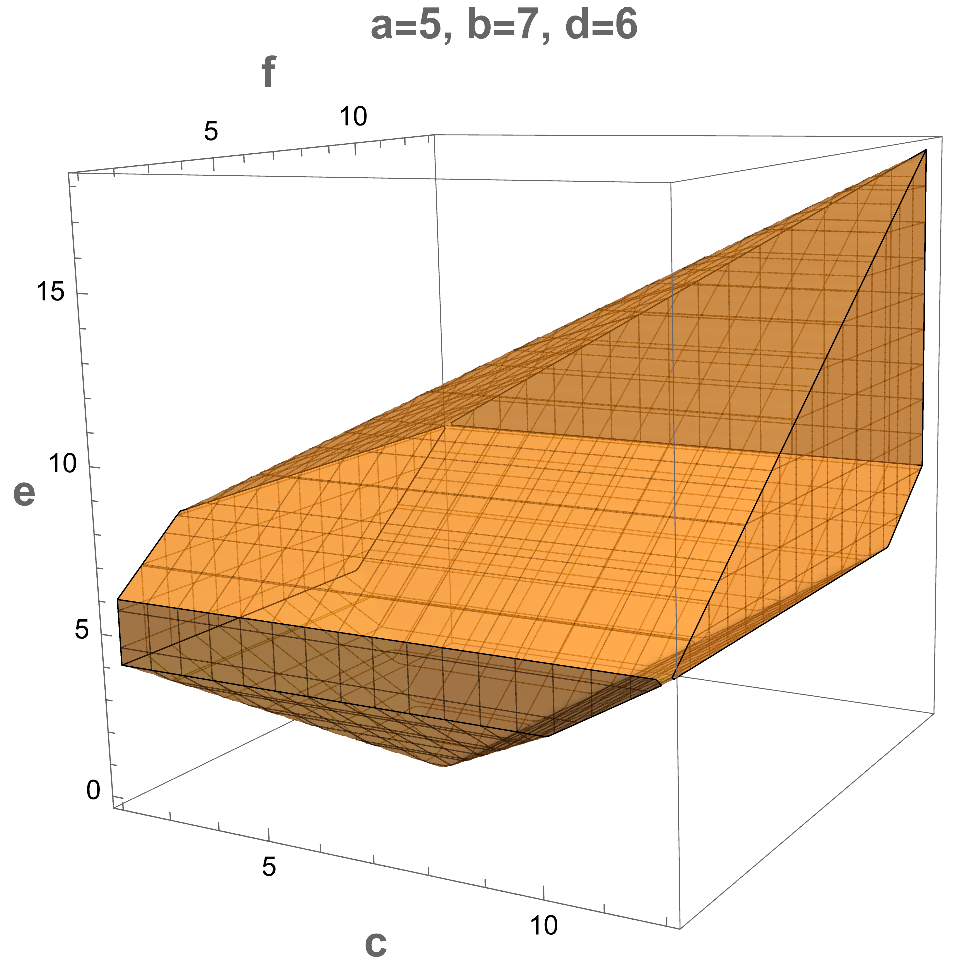
\includegraphics[width=0.25\textwidth]{figures/triangle-faces-moduli-space-example}
        \qquad
        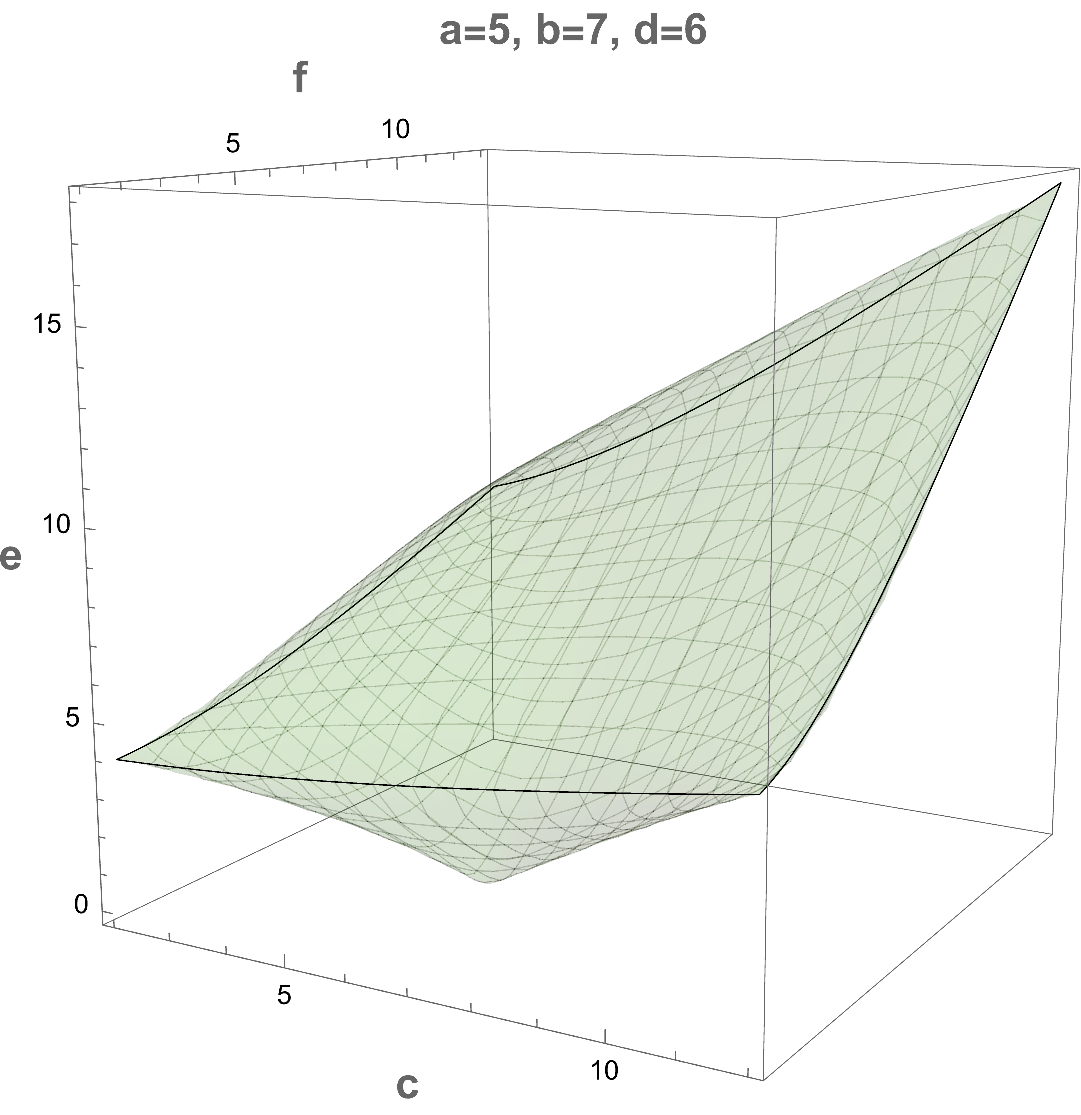
\includegraphics[width=0.25\textwidth]{figures/tetrahedron-moduli-space-example}
    \end{center}
    \caption{
        A slice of the set of admissible side-lengths $(a,b,c,d,e,f)$ for Euclidean tetrahedron along the coordinates $(a,b,d) = (5,7,6)$
        (Left) The polyhedron of values $(c, e, f)$ satisfying the triangle inequalities for each face \cref{eq:quadruplet_triangle_constraints}.
        (Right) The set of all values $(c,e,f)$ satisfying both \cref{eq:quadruplet_triangle_constraints} and \cref{eq:volume_positive_constraint}.
    }
    \label{fig:tetrahedron_moduli_space_example}
    \end{figure}
%    \begin{figure}
%        \label{fig:frustrated-tet}
%        \ctikzfig{tikz/frustrated-tetrahedron-example}
%        \caption{A example of a sextuple of edge lengths, $(a,b,c,d,e,f) = (y,y,y,x,x,x)$, which satisfies all triangle inequality constraints whenever $y \leq 2x$, but cannot be the edge lengths of any Euclidean tetrahron when $\sqrt{3} x < y$.}
%    \end{figure}
\end{exam}

\subsection{Symmetries of tetrahedral eigenvalues}
\label{sec:symmetries}

There are numerous types of symmetries present in the statement of \cref{prob:tet_problem}.
The purpose of this section is to describe the scaling, inversion, tetrahedral, and shifting symmetries of the problem.
These symmetries can, in many cases, be used to simplify the problem by selecting a canonical representative of the corresponding equivalence class; in other cases, it will be useful to leave \cref{prob:tet_problem} as stated.
%Later we will comment on the possibility of additional hidden symmetries not previously mentioned.

\begin{prop}[Scaling symmetry]
    \label{prop:scaling}
    Let $(\ea, \eb, \ec, \ed, \ee, \ef)$ be a sextuple of candidate eigenvalues and let $s \in (0, \infty)$ be a positive real number.
    Then the scaled eigenvalues, $(s\ea, s\eb, s\ec, s\ed, s\ee, s\ef)$, are tetrahedral if and only if the original, unscaled eigenvalues $(\ea, \eb, \ec, \ed, \ee, \ef)$ are tetrahedral.
\end{prop}
\begin{proof}
    The statement follows from the fact that $\eig(s X) = s \eig(X)$ holds for all Hermitian matrices $X$ and positive scalars $s$ and that each of the constraints in \cref{eq:tet_linear_constraints} are homogeneous in the six Hermitian matrices $(A,B,C,D,E,F)$; for example, we have $sA+sB-sC=0$ if and only if $s(A+B-C)=0$ if and only if $A+B-C=0$.
\end{proof}

One may wonder wether it is possible to extend the scaling symmetry to consider scaling by negative $s < 0$.
Indeed, this can be accomplished, provided one accounts for the fact that negating a Hermitian matrices both negates and reverses the order of its eigenvalues.
\begin{prop}[Inversion symmetry]
    \label{prop:inversion}
    Let $(\ea, \eb, \ec, \ed, \ee, \ef)$ be a sextuple of candidate eigenvalues.
    Given any list of non-increasing eigenvalues $\ex = (\ex_1 \geq \cdots \geq \ex_n)$, let $\ex^{*}$ denote the inverted list of resorted and negated eigenvalues: $\ex^{*} = (-\ex_d \geq \cdots \geq - \ex_1)$.
    Then $(\ea, \eb, \ec, \ed, \ee, \ef)$ are tetrahedral if and only if $(\ea^{*}, \eb^{*}, \ec^{*}, \ed^{*}, \ee^{*}, \ef^{*})$ are tetrahedral.
\end{prop}
\begin{proof}
    The statement holds because (i) $(A,B,C,D,E,F)$ satisfy \cref{eq:tet_linear_constraints} if and only if $(A',B',C',D',E',F') \coloneqq (-A,-B,-C,-D,-E,-F)$ satisfy \cref{eq:tet_linear_constraints}, and (ii) $\eig(X) = \ex$ if and only if $\eig(-X) = \ex^{*}$.
\end{proof}

The inversion symmetry \cref{prop:inversion} is just one element belonging to a group of $48$ symmetries consisting of inversions of eigenvalues, $\ex \rightarrow \ex^{*}$, or permutations of elements in the sextuple $(\ea,\eb,\ec,\ed,\ee,\ef)$.

\begin{prop}[Oriented Tetrahedral symmetry]
    \label{prop:tet_symmetry}
    The sextuple $(\ea,\eb,\ec,\ed,\ee,\ef)$ of eigenvalues are tetrahedral if and only if any (and thus all) of the following sextuples of eigenvalues are tetrahedral:
    \begin{equation}
        \label{eq:gens_of_tet_sym}
        \tightsextuple{(
            \ea & \ef  & \ee  & \ed^{*}  & \ec  & \eb
         )}
        \qquad
        \tightsextuple{(
            \ec  & \ee^*  & \ed^{*}  & \ef  & \eb  & \ea^*
        )}
    \end{equation}
    Moreover, these two operations generate a finite group of order $48$ whose action, grouped by conjugacy classes, produces:
    \begin{equation}
        \label{eq:all_of_tet_sym}
        \tightsextuple{
            (\ea  & \eb  & \ec  & \ed  & \ee  & \ef )\\[1em]
            (\ed  & \eb  & \ef  & \ea  & \ee  & \ec )\\
            (\ed^* & \ee  & \ec  & \ea^* & \eb  & \ef )\\
            (\ea  & \ee^* & \ef^* & \ed  & \eb^* & \ec^*)\\[1em]
            (\eb  & \ef^* & \ed^* & \ee  & \ec  & \ea )\\
            (\ec  & \ea^* & \eb  & \ef^* & \ed^* & \ee^*)\\
            (\ee  & \ec^* & \ed  & \eb  & \ef  & \ea^*)\\
            (\ef  & \ea  & \ee  & \ec^* & \ed  & \eb^*)\\
            (\ef^* & \ed  & \eb^* & \ec  & \ea  & \ee )\\
            (\ee^* & \ef  & \ea^* & \eb^* & \ec^* & \ed )\\
            (\ec^* & \ed^* & \ee^* & \ef  & \ea^* & \eb )\\
            (\eb^* & \ec  & \ea  & \ee^* & \ef^* & \ed^*)\\
        }
        \quad
        \tightsextuple{
            (\ea ^* & \ec  & \eb  & \ed  & \ef  & \ee )\\
            (\eb ^* & \ea ^* & \ec ^* & \ee  & \ed  & \ef )\\
            (\ef ^* & \eb  & \ed ^* & \ec ^* & \ee ^* & \ea ^*)\\
            (\ee  & \ed ^* & \ec  & \eb ^* & \ea  & \ef ^*)\\
            (\ec  & \eb ^* & \ea  & \ef  & \ee  & \ed )\\
            (\ea  & \ef  & \ee  & \ed ^* & \ec  & \eb )\\[2em]
            (\eb  & \ed  & \ef  & \ee^* & \ea^* & \ec^*)\\
            (\ed  & \ef^* & \eb^* & \ea^* & \ec^* & \ee^*)\\
            (\ef  & \ee^* & \ea^* & \ec  & \eb  & \ed^*)\\
            (\ee^* & \ea  & \ef^* & \eb  & \ed^* & \ec )\\
            (\ed^* & \ec^* & \ee^* & \ea  & \ef^* & \eb^*)\\
            (\ec^* & \ee  & \ed  & \ef^* & \eb^* & \ea )\\
        }
        \quad
        \tightsextuple{
            (\ea  & \ec ^* & \eb ^* & \ed ^* & \ef ^* & \ee ^*)\\
            (\eb  & \ea  & \ec  & \ee ^* & \ed ^* & \ef ^*)\\
            (\ef  & \eb ^* & \ed  & \ec  & \ee  & \ea )\\
            (\ee ^* & \ed  & \ec ^* & \eb  & \ea ^* & \ef )\\
            (\ec ^* & \eb  & \ea ^* & \ef ^* & \ee ^* & \ed ^*)\\
            (\ea ^* & \ef ^* & \ee ^* & \ed  & \ec ^* & \eb ^*)\\[2em]
            (\eb^* & \ed^* & \ef^* & \ee  & \ea  & \ec )\\
            (\ed^* & \ef  & \eb  & \ea  & \ec  & \ee )\\
            (\ef^* & \ee  & \ea  & \ec^* & \eb^* & \ed )\\
            (\ee  & \ea^* & \ef  & \eb^* & \ed  & \ec^*)\\
            (\ed  & \ec  & \ee  & \ea^* & \ef  & \eb )\\
            (\ec  & \ee^* & \ed^* & \ef  & \eb  & \ea^*)\\
        }
        \quad
        \tightsextuple{
            (\ea^* & \eb^* & \ec^* & \ed^* & \ee^* & \ef^*)\\[1em]
            (\ed^* & \eb^* & \ef^* & \ea^* & \ee^* & \ec^*)\\
            (\ed  & \ee^* & \ec^* & \ea  & \eb^* & \ef^*)\\
            (\ea^* & \ee  & \ef  & \ed^* & \eb  & \ec )\\[1em]
            (\eb^* & \ef  & \ed  & \ee^* & \ec^* & \ea^*)\\
            (\ec^* & \ea  & \eb^* & \ef  & \ed  & \ee )\\
            (\ee^* & \ec  & \ed^* & \eb^* & \ef^* & \ea )\\
            (\ef^* & \ea^* & \ee^* & \ec  & \ed^* & \eb )\\
            (\ef  & \ed^* & \eb  & \ec^* & \ea^* & \ee^*)\\
            (\ee  & \ef^* & \ea  & \eb  & \ec  & \ed^*)\\
            (\ec  & \ed  & \ee  & \ef^* & \ea  & \eb^*)\\
            (\eb  & \ec^* & \ea^* & \ee  & \ef  & \ed )\\
        }
    \end{equation}
\end{prop}
\begin{proof}
    To begin, notice that each of the operations on $(\ea,\eb,\ec,\ed,\ee,\ef)$ appearing in \cref{eq:gens_of_tet_sym} are invertible (indeed the first operation has order two, while the second operation has order four).
    The claim that these two operations generate a finite group of order $48$ can be checked explicitly using computer software.
    Now suppose $(\ea,\eb,\ec,\ed,\ee,\ef)$ are the eigenvalues of a sextuple of Hermitian matrices $(A,B,C,D,E,F)$ satisfying \cref{eq:tet_linear_constraints}.
    Then, for example, the sextuple $(A',B',C',D',E',F') = (A,F,E,-D,C,B)$ (which has the eigenvalues $(\ea, \ef, \ee, \ed^{*}, \ec, \eb)$) is also tetrahedral because
    \begin{align}
        \label{eq:signed_perm_rows}
        \begin{split}
            A'+B'-C' &= (A+F-E) = 0,  \\
            B'+D'-F' &= -(B+D-F) = 0, \\
            C'+D'-E' &= -(C+D-E) = 0, \\
            A'+F'-E' &= (A+B-C) = 0.
        \end{split}
    \end{align}
    Moreover, as the operation mapping $(\ea,\eb,\ec,\ed,\ee,\ef)$ to $(\ea^*, \ec, \eb, \ed, \ef, \ee)$ is invertible, one also has that if $(\ea,\eb,\ec,\ed,\ee,\ef)$ is not tetrahedral, then neither is $(\ea^*, \ec, \eb, \ed, \ef, \ee)$.
    An analogous argument holds for the operation mapping $(\ea,\eb,\ec,\ed,\ee,\ef)$ to $(\ec, \ee^*, \ed^{*}, \ef, \eb, \ea^*)$ with $(A',B',C',D',E',F')$ given by $(C,-E,-D,F,B,-A)$.
\end{proof}
\begin{prop}[Shifting symmetry]
    \label{prop:shifting}
    Let $(\ea, \eb, \ec, \ed, \ee, \ef)$ be a sextuple of candidate eigenvalues and let $x,y,z \in \mathbb R$ be fixed.
    Given any list of non-increasing eigenvalues $\ex = (\ex_1 \geq \cdots \geq \ex_n)$, let $\ex + x \coloneqq (\ex_1 + x \geq \cdots \geq \ex_d + x)$.
    Then define shifted eigenvalues by the formula
    \begin{equation}
        \label{eq:shifted_tet_eigenvalues}
        \begin{alignedat}{3}
             &\tilde \ea     \coloneqq \ea + x, \qquad
            &&\tilde \eb      \coloneqq \eb + y, \qquad
            &&\tilde \ec     \coloneqq \ec + x + y, \\
             &\tilde \ed     \coloneqq \ed + z, \qquad
            &&\tilde \ee   \coloneqq \ee + x + y + z, \qquad
            &&\tilde \ef       \coloneqq \ef + y + z.
        \end{alignedat}
    \end{equation}
    The shifted eigenvalues $(\tilde \ea, \tilde \eb, \tilde \ec, \tilde \ed, \tilde \ee,\tilde \ef)$ are tetrahedral if and only if the unshifted eigenvalues $(\ea, \eb, \ec, \ed, \ee, \ef)$ are tetrahedral.
\end{prop}
\begin{proof}
    Given a Hermitian matrix $X$ with eigenvalues $\eig(X) = \ex$ and a constant $w \in \mathbb R$, the eigenvalues of $X+wI$ (where $I$ is the identity matrix) are
    \begin{equation}
        \eig(X+wI) = \ex + w = (\ex_1 + w \geq \cdots \geq \ex_d + w).
    \end{equation}
    The statement then follows because
    \begin{equation}
        (A+xI,B+yI,C+(x+y)I,D+zI, E+(x+y+z)I, F+(y+z)I)
    \end{equation}
    satisfy the tetrahedral constraints in \cref{eq:tet_linear_constraints} if and only if $(A,B,C,D,E,F)$ satisfy the tetrahedral constraints in \cref{eq:tet_linear_constraints}
\end{proof}
As a corollary of the shifting symmetries (\cref{prop:shifting}) one concludes that to solve the tetrahedral Horn's problem, in a certain sense, it suffices to solve the tetrahedral Horn's problem merely for traceless matrices (\cref{cor:traceless}) or, alternatively, for positive definite or positive semidefinite matrices (\cref{cor:psd}).
\begin{cor}[Traceless eigenvalues]
    \label{cor:traceless}
    Let $(\ea, \eb, \ec, \ed, \ee, \ef)$ be a sextuple of candidate eigenvalues and for any list of $n$ eigenvalues $\ex = (\ex_1 \geq \cdots \geq \ex_n)$, let $\ex^{0} \coloneqq \ex - {\tex}/n$ denote the traceless list of eigenvalues obtained by shifting $\ex$ by $-{\tex}/n$.
    Then $(\ea, \eb, \ec, \ed, \ee, \ef)$ are tetrahedral if and only if (i) their traces $({\tea}, {\teb}, {\tec}, {\ted}, {\tee}, {\tef})$ are tetrahedral (they satisfy \cref{eq:tet_trace_conds}) and (ii) $(\ea^0, \eb^0, \ec^0, \ed^0, \ee^0, \ef^0)$ are tetrahedral.
\end{cor}
\begin{proof}
    This ``only if'' portion of the statement follows from both the tetrahedral trace conditions (\cref{eq:tet_trace_conds}) and applications of the shifting symmetry \cref{prop:shifting} with $(x,y,z)$ values
    \begin{equation}
        x = - n^{-1}\Tr(A), \qquad
        y = - n^{-1}\Tr(B) \qquad
        z = - n^{-1}\Tr(D).
    \end{equation}
    The ``if'' portion of the statement follows from the shifting symmetry applied to the negated $(x,y,z)$ values.
\end{proof}
The next corollary of the shifting symmetry proves that to solve the tetrahedral Horn's problem it suffices to solve the tetrahedral Horn's problem for positive definite spectra only.
Indeed, one can simply take the shifting parameters $(x,y,z)$ appearing in \cref{prop:shifting} to be sufficiently large.
The following corollary establishes, in a certain sense, the minimum shifting required to ensure strictly positive eigenvalues for all six Hermitian matrices.
Note that in subsequent sections we will often explicitly assume the candidate eigenvalues $(\ea,\eb,\ec,\ed,\ee,\ed)$ are either non-negative or positive for the sake of technical convenience or sometimes to establish a connection with density matrices from quantum theory (which are positive semidefinite matrices with unit trace).
\begin{cor}[Positive eigenvalues]
    \label{cor:psd}
    If $(\ea, \eb, \ec, \ed, \ee, \ef)$ are a tetrahedral sextuple of eigenvalues, then necessarily the smallest eigenvalues satisfy
    \begin{equation}
        \label{eq:min_eig_ineqs}
        \ec_d \geq \ea_d + \eb_d, \qquad \ef_d \geq \eb_d + \ed_d, \qquad \ee_d \geq \ed_d + \ec_d, \qquad \ee_d \geq \ea_d + \ef_d.
    \end{equation}
    Moreover, if $(\ea, \eb, \ec, \ed, \ee, \ef)$ are a sextuple of candidate eigenvalues satisfying \cref{eq:min_eig_ineqs}, then for any $(x,y,z) \in \mathbb R^{3}$ satisfying
    \begin{equation}
        \label{eq:positive_shift}
        x > -\ea_d, \qquad
        y > -\eb_d, \qquad
        z > -\ed_d,
    \end{equation}
    the resulting shifted eigenvalues $(\tilde \ea, \tilde \eb, \tilde \ec, \tilde \ed, \tilde \ee, \tilde \ef)$ (given by \cref{eq:shifted_tet_eigenvalues}) are all positive.
\end{cor}
\begin{proof}
    That tetrahedral eigenvalues satisfy \cref{eq:min_eig_ineqs} follows from four applications of the well-known inequality $\ec_d \geq \ea_d + \eb_n$ for Horn's problem where $C=A+B$ \cite{bhatia2001linear}.
    As a reminder, the smallest eigenvalue $\ex_n$ of a matrix $X$ is characterized by a minimization: $\ex_d = \min_{\norm{v} = 1} \braket{v, Xv}$ which produces
    \begin{equation}
        \ec_d = \min_{\norm{v} = 1} \braket{v, C v} = \min_{\norm{v} = 1} \left(\braket{v, A v} + \braket{v, B v}\right) \geq \min_{\norm{v} = 1} \braket{v, A v} + \min_{\norm{w} = 1}\braket{w, B w} = \ea_d + \eb_d.
    \end{equation}
    Four applications of this inequality produces \cref{eq:min_eig_ineqs}.
    Now if $(x,y,z)$ satisfy \cref{eq:positive_shift}, we have for all $j$
    \begin{equation}
        \ea_j + x \geq \ea_d + x > 0,
    \end{equation}
    meaning $\ea+x = (\ea_1 + x \geq \cdots \geq \ex_d + x)$ is strictly positive.
    Similar statements hold for $\eb,\ec,\ed, \ee$ and $\ef$; for instance, for all $j$,
    \begin{equation}
        \ee_j + x + y + z \geq \ee_d + x + y + z > \ee_d - \ea_d - \eb_d - \ed_d \geq 0,
    \end{equation}
    meaning $\ee+x+y+z$ is strictly positive also.
\end{proof}

\begin{rem}
    Although this section listed a handful of symmetries of the tetrahedral Horn's problem, there remains the possibility of additional symmetries which are unknown at this time.
    For example, in the case $2\times 2$ Hermitian matrices, an additional class of symmetries on the set of edge-lengths $(a,b,c,e,d,f)$ of tetrahedra, known as the \textit{Regge symmetries}, hold \cite[Theorem 1.1]{akopyan2019regge,boalch2007regge,ponzano1968semiclassical}.
    If there exists a tetrahedron with edge lengths $(a,b,c,d,e,f)$, then there also exists a tetrahedron with edge lengths
    \begin{equation}
        (s_1-a,s_1-b,c,s_1-d,s_1-e,f) \quad \text{where} \quad s_1 = \frac{a+b+d+e}{2}.
    \end{equation}
    Combining this symmetry with the permutational symmetries given by \cref{prop:tet_symmetry} (and noting that for the eigenvalues $\ex$ of traceless $2 \times 2$ Hermitian matrices, $\ex = (x, -x)$, we have $\ex^{*} = \ex$) one concludes the co-existence of a family of six tetrahedra with edge lengths given by \cite[Chapter 9]{varshalovich1988quantum}:
    \begin{equation}
        \begin{alignedat}{2}
            &(a,b,c,d,e,f) \quad
            &&(s_1-a,s_1-b,c,s_1-d,s_1-e,f) \\
            &(a,s_3-b,s_3-c,d,s_3-e,s_3-f) \quad
            &&(s_2-a,b,s_2-c,s_2-d,e,s_2-f) \\
            &(s_2-d,s_1-e,s_3-f,s_2-a,s_1-b,s_3-c) \quad
            &&(s_1-d,s_3-e,s_2-f,s_1-a,s_3-b,s_2-c)
        \end{alignedat}
    \end{equation}
    where
    \begin{equation}
        s_1 = \frac{a+b+d+e}{2}, \quad
        s_2 = \frac{a+c+d+f}{2}, \quad
        s_3 = \frac{b+c+e+f}{2}.
    \end{equation}
\end{rem}
\begin{rem}
    The Regge symmetry of a tetrahedron can be understood as a consequence of an earlier discovery of a suprisinging symmetry of Wigner $6j$ symbol for $\SU(2)$ originally due to \citeauthor{regge1959symmetry} \cite{regge1959symmetry}.
    The paper due to \citeauthor{boalch2007regge} provides a comphrehensive and modern treatment of the Regge symmetry for the $6j$ symbol for $\SU(2)$ by viewing it as a consequence of a simpler symmetry of the $6j$-symbol for $\SU(3)$ \cite{boalch2007regge}.
    That the Regge symmetry of a tetrahedron emerges from the Regge symmetry of the associated $6j$ symbols can be viewed as a consequence of the semiclassical limit of the latter \cite{ponzano1968semiclassical,roberts1999classical}.
    It has also be shown that the Regge symmetry of Euclidean tetrahedra is actually a scissors-congruence preserving both the volume and Dhen invariants \cite{akopyan2019regge}.

    At the moment, it remains unclear if there exists analogous symmetries for the generalized Wigner $6j$ symbol for $n \geq 3$ (although there are conjectured symmetries for the $6j$ symbols for $U_q(\mathfrak{sl}_n)$ which would follow from the eigenvalue hypothesis \cite{morozov2018new,lanina2023tug}).
    It could also be possible for additional symmetries to be present in the tetrahedral Horn problem for $n \geq 3$ which are \textit{not} present in the $6j$ symbol for $\SU(n)$.
\end{rem}

\clearpage
\section{Polynomial inequalities}

The eigenvalues, $\ex = (\ex_1, \ldots, \ex_n)$, of an $n \times n$ Hermitian matrix $X$ determine which $\U(n)$ orbit,

\subsection{Polynomial representations \& Schur-Weyl duality}

The purpose of this section is to review the representation theory of $\U(n)$, or equivalently, the polynomial representation theory of $\GL(n)$.

will be to examine the Schur-Weyl decomposition of the $k$-th tensor power $A^{\ot k}$.
To begin, we recall the Schur-Weyl decomposition of $(\mathbb C^{n})^{\ot k}$ as a representation of the group $S_k \times \U(n)$.

\begin{prop}[Schur-Weyl duality]
    Let $k$ and $n$ be positive integers.
    Then the decomposition of $(\mathbb C^{n})^{\ot k}$ into irreducible subrepresentations of $S_k \times \U(n)$, known as the \textit{Schur-Weyl} decomposition, is given by
    \begin{equation}
        \label{eq:schur_weyl_decomp}
        (\mathbb C^{n})^{\ot k} \cong \bigoplus_{\yx \vdash_{n} k} W_{\yx} \ot V_{\yx}^{n}
    \end{equation}
    where the direct summands are indexed by Young diagrams $\yx$ with $k$ boxes and at most $n$ rows, and where $W_{\yx}$ supports the irreducible representation of $S_k$ and $V_{\yx}^{n}$ supports the irreducible representation of $\U(n)$.
\end{prop}

The dimension of the $V_{\yx}^n$ is given by Weyl's dimension formula \cite{hall2008representations,itzykson1966unitary},
\begin{equation}
    \label{eq:weyl_dim}
    \dim(V_{\yx}^{n}) = \frac{\Delta_n(\tilde \yx)}{\Delta_n(\rho)},
\end{equation}
whereas the dimension of $W_{\yx}$ may be given by \cite[Corollary 9.1.5]{goodman2000representations},
\begin{equation}
    \label{eq:frob_dim}
    \dim(W_{\yx}) = \frac{{\syx}!}{\tilde \yx_1!\tilde \yx_2! \cdots \tilde \yx_n!} \Delta_n(\tilde \yx)
\end{equation}
where $\tilde \yx = \yx + \rho$, where $\rho =(n-1, n-2, \ldots, 1, 0)$ is known as the Weyl vector and where $\Delta_n(x_1, \ldots, x_n) = \prod_{1 \leq i < j \leq n} (x_i-x_j)$ is the Vandermonde determinant.
Note that the representation $W_{\yx}$ of $S_{k}$ is independent of $n$;
indeed, the right hand side of \cref{eq:frob_dim} does not depend on $n$ and coincides with the Hook-length formula \cite[Corollary 9.1.6]{goodman2000representations} (any value of $n$ which is at least the depth of $\yx$ suffices).

\begin{defn}
    Given a non-zero positive semidefinite $n \times n$ matrix $A$, a positive integer $x$, and a Young diagram $\ya \vdash_n x$, let
    \begin{equation}
        \tau_{\ya}(A) 
        \coloneqq \Tr[\nrm A^{\ot a} P_{\ya}],
    \end{equation}
    where $\nrm A = \frac{A}{\Tr(A)}$ is the normalization of $A$ and $P_{\ya}$ projects onto the isotypic component of $(\mathbb C^n)^{\ot a}$ indexed by $\ya$.
\end{defn}
As $P_{\ya}$ is $\U(n)$-equivariant, one observes that $\tau_{\ya}(A)$ depends only on the eigenvalues of $A$.
The following result, know as spectrum or eigenvalue estimation, states that the map $\ya \mapsto \tau_{\ya}(A)$ for $A$ positive semidefinite is concentrated those Young diagrams $\ya$ whose shape matches the shape of the eigenvalues $\ea = \eig(A)$ \cite{alicki1988symmetry,keyl2001estimating,hayashi2002quantum}.
\begin{prop}[Eigenvalue estimation]
    \label{prop:eig_est}
    Let $A$ be a positive semidefinite matrix with eigenvalues $\ea = \eig(A)$ and let $\ya \vdash_n a$.
    Then
    \begin{equation}
        \tau_{\ya}(A) \leq \dim(V_{\ya}^{n}) \exp(-a \kl{\nya}{\nea}),
    \end{equation}
    where $\kl{\nya}{\nea}$ denotes the Kullback-Leibler divergence of $\nya$ from $\nea$.
\end{prop}
\begin{proof}
    See \cite{keyl2001estimating} for a proof (noting that $\Tr(\nrm A) = 1$).
\end{proof}
\begin{prop}
    \label{prop:completeness_rel_uni}
    Let $A$ be positive semidefinite $n\times n$ matrix with $\Tr(A) = 1$ with eigenvalues $\ea = \eig(A)$ and rank $r(\ea) = \rank(A)$.
    Then for any positive integer $a$,
    \begin{equation}
        \sum_{\ya \vdash_{r(\ea)} a} \tau_{\ya}(A) = 1,
    \end{equation}
    where the sum if over Young diagrams $\ya$ with size $a$ with depth at most $r(\ea)$.
\end{prop}

\begin{defn}
    Let $(\pi_{\yx}, V_{\yx}^n)$ be an irreducible representation of $\U(n)$ labelled by the Young diagram $\yx$.
    Given an $n \times n$ matrix $X$, viewed as a linear operator on the defining representation $V_{(1)}^{n} \simeq \mathbb C^{n}$, we define $\pi_{\yx}(X)$ by the formula:
    \begin{equation*}
        \pi_{\yx}(X) \coloneqq \frac{\Tr_{W_{\yx}}[\iota_{\yx}^{\dagger} X^{\ot {\syx}} \iota_{\yx}]}{\dim(W_{\yx})}
    \end{equation*}
    where $\iota_{\yx} : W_{\yx} \ot V_{\yx}^{n} \to V_{(1)}^{\ot {\syx}}$ is the equivariant isometry for the $\yx$-isotypic subspace of $V_{(1)}^{\ot {\syx}}$.
    This definition ensures that $X^{\ot k} \simeq \bigoplus_{\yx \vdash k} \pi_{\yx}(X)^{\oplus W_{\yx}}$ holds for any positive integer $k$.
    When $X$ is a unitary, $\pi_{\yx}(X)$ is the representation of $X$ on $V_{\yx}^{n}$, so this abuse of notation is warranted.
    If $X \geq 0$ is positive semidefinite, then $\pi_{\yx}(X) \geq 0$ is positive semidefinite also.
    If $\yx = (1)$, then $\pi_{(1)}(X) = X$ as $\dim(W_{(1)}) = 1$.

    Note also that the matrix coefficients of $\pi_{\yx}(X)$ are homogeneous degree $\abs{\lambda}$ polynomials in the matrix coefficients of $X$ meaning for any scalar $s \in \mathbb C$,
    \begin{equation}
        \pi_{\yx}(sX) = s^{{\syx}} \pi_{\yx}(X).
    \end{equation}
    Additionally, if $X,Y$ are two matrices, we have
    \begin{equation}
        \pi_{\yx}(XY) = \pi_{\yx}(X)\pi_{\yx}(Y). 
    \end{equation}
    The \textit{character} of $X$ satisfies
    \begin{equation*}
        \chi_{\yx}(X) \coloneqq \Tr(\pi_{\yx}(X)) = \frac{\Tr[P_{\yx} X^{\ot {\syx}}]}{\dim(W_{\yx})} = s_{\yx}(\eig(X)),
    \end{equation*}
    where $s_{\yx}(\eig(X))$ is the corresponding Schur-polynomial evaluated on the eigenvalues of $X$.
    For fixed positive integer $k$, we also define the \textit{Plancherel distribution} $\{\mu_\yx | \yx \vdash k\}$ over Young diagrams of size $k$ according to
    \begin{equation}
        \mu_\yx \coloneqq \frac{(\dim W_\yx)^2}{{\syx}!}.
    \end{equation}
    Moreover, we define the rescaling of $\pi_{\yx}(X)$ to be
    \begin{equation*}
        \tilde \pi_{\yx}(X) \coloneqq \dim(W_{\yx}) \pi_{\yx}(X) = \Tr_{W_{\yx}}[\iota_{\yx}^{\dagger} X^{\ot {\syx}} \iota_{\yx}],
    \end{equation*}
    and the corresponding rescaled character is
    \begin{equation*}
        \tilde \chi_\yx(X) \coloneqq \Tr[\tilde \pi_{\yx}(X)] = \Tr[P_{\yx} X^{\ot {\syx}}] = \dim(W_{\yx})s_{\yx}(\eig(X)),
    \end{equation*}
    where $P_{\yx} \coloneqq \iota_{\yx}^{\dagger} \iota_{\yx}$ is the orthogonal projection operator onto the $\yx$-isotypic subspace.

    These rescaled characters emerge as coefficients in the following decomposition associated to an integral over Haar measure over $\U(n)$,
    \begin{equation}
        \int_{\U(n)} \diff U (U X U^{-1})^{\ot k} = \sum_{\lambda \vdash k} \tilde \chi_{\yx}(X)   \frac{P_{\yx}}{\Tr(P_{\yx})}.
    \end{equation}
    This normalization scheme means that $\tilde \pi_{\yx}(X)$ is \textit{not} a representation, while the character $\tilde \chi_{\yx}(X)$ satisfies
    \begin{equation}
        \sum_{\yx \vdash k} \tilde \chi_{\yx}(X) = \sum_{\yx \vdash k} \Tr[X^{\ot k} P_{\yx}] = \Tr[X^{\ot k}] = \Tr[X]^k.
    \end{equation}
    Therefore, whenever $X$ is positive semidefinite and trace one (i.e., when $X$ is a density matrix), we have that the map $\yx \mapsto \tilde \chi_{\yx}(X)$ is a probability distribution when restricted to the set of Young diagrams with a fixed number $k$ of boxes:
    \begin{equation}
        X\geq 0 \implies \tilde \chi_{\yx}(X) \geq 0, \qquad \text{and} \qquad \Tr(X) = 1 \implies \sum_{\yx \vdash k} \tilde \chi_{\yx}(X) = 1.
    \end{equation}
    As the (rescaled) character $\chi_{\yx}(X)$ depends only on the eigenvalues $\eig(X)$ of $X$, we have
    \begin{equation}
        \chi_{\yx}(X) = \chi_{\yx}(\diag(\eig(X)).
    \end{equation}
    Given a tuple of non-negative sorted eigenvalues $\ex = (\ex_1 \geq \cdots \geq \ex_n \geq 0)$ summing to one, $\sum_{i=1}^{n}\ex_i = 1$, the distribution $\yx \mapsto \tilde \chi_{\yx}(\diag(\ex))$ over $\yx \vdash k$ is denoted $\mathrm{SW}^{k}(\ex)$ and called the \textit{Schur-Weyl} distribution in \cite{odonnell2016efficient}.
\end{defn}

\subsection{The binomial theorem}
\label{sec:binomial_theorem}

The purpose of this section is to state and prove a the binomial theorem, which serves as the foundation for all subsequent results in this paper.
The binomial theorem expresses any polynomial irreducible representation of a matrix sum $X+Y$ as a sum over the polynomial irreducible representations of the summands $X$ and $Y$.

The theorem inherits its name from the non-commutative binomial expansion of the $k$-th tensor power of the sum $X+Y$,
\begin{equation}
    (X+Y)^{\ot k} = \sum_{\ell=0}^{k} \binom{k}{\ell} \left[\frac{1}{k!} \sum_{\sigma \in S_{k}} \sigma (X^{\ot \ell} \otimes Y^{\ot (k - \ell)})\sigma^{-1}\right]
\end{equation}
where $\sigma \in S_{k}$ acts on $(\mathbb C^{n})^{\ot k}$ by permutation of the $k$ tensor factors.
For an example, consider the case where $k=3$:
\begin{align}
    \begin{split}
        (X+Y)^{\ot 3} 
        &= \underbrace{X \ot X \ot X}_{\ell=3} + \underbrace{X \ot X \ot Y + X \ot Y \ot X + Y \ot X \ot X}_{\ell=2} + \\
        &\qquad + \underbrace{X \ot Y \ot Y + Y \ot X \ot Y + Y \ot Y \ot X}_{\ell=1}  + \underbrace{Y \ot Y \ot Y}_{\ell=0}.
    \end{split}
\end{align}
As we have seen previously, the $k$-th tensor power of a matrix can also be decomposed into a sum over polynomial irreducible representations labelled by Young diagrams $\yc$ with sizes $\syc = k$.
Combining this formula with the non-commutative binomial expansion yields
\begin{equation}
    (X+Y)^{\ot k} = \sum_{\yc \vdash k} \iota_{\yc} (\pi_{\yc}(X+Y) \ot \id_{W_{\yc}}) \iota_{\yc}^{\dagger}
\end{equation}
where
\begin{equation}
    \pi_{\yc}(X+Y) = \frac{1}{\dim (W_{\yc})} \sum_{\ell=0}^{k} \binom{k}{\ell} \Tr_{W_{\yc}}[\iota_{\yc}^{\dagger} (X^{\ot \ell} \otimes Y^{\ot (k - \ell)}) \iota_{\yc}],
\end{equation}
where we have eliminated the symmetrization operation over $\sigma \in S_k$ because the partial trace over $W_{\yc}$ is $S_k$-invariant.
At this stage, for each summand indexed by $0 \leq \ell \leq k$, we can decompose $X^{\ot \ell}$ into representations of $X$ labelled by $\ya$ with sizes $\sya = \ell$ and $Y^{\ot \ell}$ into representations of $Y$ labelled by $\yb$ with sizes $\syb = k-\ell$.
\begin{align}
    X^{\ot \ell} = \sum_{\ya \vdash \ell} \iota_{\ya} (\pi_{\ya}(X) \ot \id_{W_{\ya}}) \iota_{\ya}^{\dagger}, \qquad
    Y^{\ot k-\ell} = \sum_{\yb \vdash k-\ell} \iota_{\yb} (\pi_{\yb}(Y) \ot \id_{W_{\yb}}) \iota_{\yb}^{\dagger}.
\end{align}
Upon doing so, one encounters the composite operator $\iota_{\yc}^{\dagger}(\iota_{\ya} \ot \iota_{\yb})$ which maps from $(V_{\ya}^{n} \ot W_{\ya}) \ot (V_{\yb}^{n} \ot W_{\yb})$ to $(V_{\yc}^{n} \ot W_{\yc})$ in an $S_\ell \times S_{k-\ell}$-equivariant and $\U(n)$-equivariant manner.
By Schur's lemma and Schur-Weyl duality, it can be written as
\begin{equation}
    \iota_{\yc}^{\dagger}(\iota_{\ya} \ot \iota_{\yb}) = (\id_{V_{\yc}^{n}} \ot \omega^{\yc}_{\ya\yb}) (\iota^{\yc}_{\ya\yb} \ot \id_{W_{\ya} \ot W_{\yb}})^{\dagger}
\end{equation}
where $\iota^{\yc}_{\ya\yb} : C^{\yc}_{\ya\yb} \ot V_{\yc}^{n} \to V_{\ya}^{n} \ot V_{\yb}^{n}$ is the $\U(n)$-equivariant isometry for the $\yc$-isotypic subspace of $V_{\ya}^{n}\ot V_{\yb}^{n}$ and $\omega^{\yc}_{\ya\yb} : C^{\yc}_{\ya\yb} \ot W_{\ya} \ot W_{\yb} \to W_{\yc}$ the $S_\ell \times S_{k-\ell}$-equivariant isometry for the $(\ya,\yb)$-isotypic subspace of $W_{\yc}$.\footnote{Schur-Weyl duality provides us with a isometric and bijective identification between the multiplicity spaces for $V_{\yc}^{n}$ inside $V_{\ya}^{n} \ot V_{\yb}^{n}$ with respect to $U(n)$ and $W_{\ya} \ot W_{\yb}$ inside $W_{\yc}$ with respect to $S_{\ell} \times S_{k-\ell}$, hence why we use, by abuse of notation, the symbol $C^{\yc}_{\ya\yb}$ in both cases.}
Combining everything together, and rearranging we obtain the formula
\begin{equation}
    \label{eq:proto_binomial_theorem}
    \frac{\dim W_{\yc} \pi_{\yc}(X+Y)}{\syc!} = \sum_{\ya,\yb} \Tr_{C^{\yc}_{\ya,\yb}} \left[ (\iota^{\yc}_{\ya,\yb})^{\dagger} \frac{\dim W_{\ya} \pi_{\ya}(X)}{\sya!} \ot \frac{\dim W_{\ya} \pi_{\yb}(Y)}{\syb!} (\iota^{\yc}_{\ya,\yb})\right],
\end{equation}
where we leave the summation over all pairs $(\ya,\yb)$ such that $\sya = \ell$, $\syb = k -\ell$ for $\syc = k$ implicit simply because the multiplicity space $C^{\yc}_{\ya\yb}$ is empty if $\sya + \syb \neq \syc$ and thus the corresponding summand is taken to be zero.

In the remaining of the paper, we will use the above formula, \cref{eq:proto_binomial_theorem}, to prove numerous results concerning the eigenvalues of Hermitian matrices and their sums.
In order to simplify the presentation of our results considerably, we introduce the following definitions.
\begin{defn}[Hook-rescaled representations]
    Given an $n\times n$ matrix $X$ and a Young diagram $\yx$, define an operator $\Phi_{\yx}(X)$ acting on the representation space $V_{\yx}^{n}$ as any of the following equivalent expressions:
    \begin{equation}
        \Phi_{\yx}(X) \coloneqq \frac{\dim W_{\yx} \pi_{\yx}(X)}{\syx!} = \frac{\pi_{\yx}(X)}{H_{\yx}} = \frac{\Tr_{W_{\yx}}[\iota_{\yx} X^{\ot \syx} \iota_{\yx}^{\dagger}]}{\syx!},
    \end{equation}
    where $H_{\yx} = \prod_{b\in\yx} h_{\yx}(b)$ is the product of the Hook-lengths of the boxes in the Young diagram $\yx$.
    Furthermore, let the trace of $\Phi_{\yx}(X)$ be denoted by
    \begin{equation}
        \varphi_{\yx}(X) = \Tr[\Phi_{\yx}(X)] = \frac{\dim W_{\yx} \chi_{\yx}(X)}{\syx!} = \frac{\chi_{\yx}(X)}{H_{\yx}} = \frac{\Tr[P_{\yx} X^{\ot \syx}]}{\syx!}.
    \end{equation}
\end{defn}

\begin{rem}
    The operator $\Phi_{\yx}(X)$ and trace $\varphi_{\yx}(X)$ are simply rescalings of the representation matrix $\pi_{\yx}(X)$ of $X$ and the character $\chi_{\yx}(X)$ of $X$ respectively.
    This normalization scheme is such that summing the rescaled character over all Young diagrams $\yx$ with fixed size $k$ or over all sizes yields respectively
    \begin{equation}
        \sum_{\yx \vdash k} \varphi_{\yx}(X) = \frac{\Tr(X)^k}{k!},
        \qquad
        \sum_{\yx} \varphi_{\yx}(X) = \exp(\Tr(X)).
    \end{equation}
\end{rem}

Before stating the main result of this section, we first generalize the quantities $\Phi_{\yx}(X)$ and $\varphi_{\yx}(X)$ to consider arguments involving more than one matrix.

\begin{defn}[Mixed hook-rescaled representations]
    Given a pair $(X,Y)$ of $n\times n$ matrices and a triple of Young diagrams $(\ya,\yb,\yc)$, define an operator $\Phi^{\ya\yb}_{\yc}(X,Y)$ acting on the representation space $V_{\yc}^{n}$ as
    \begin{equation}
        \Phi^{\ya\yb}_{\yc}(X,Y) \coloneqq \Tr_{C^{\yc}_{\ya,\yb}} [\iota^{\yc;\dagger}_{\ya,\yb} (\Phi_{\ya}(X) \ot \Phi_{\yb}(Y)) \iota^{\yc}_{\ya,\yb}],
    \end{equation}
    where $\iota^{\yc}_{\ya\yb} : C^{\yc}_{\ya\yb} \ot V_{\yc}^{n} \to V_{\ya}^{n} \ot V_{\yb}^{n}$ is the $\U(n)$-equivariant isometry for the $\yc$-isotypic subspace of $V_{\ya}^{n} \ot V_{\yb}^{n}$.
    Note the sum over Young diagrams $\ya$, and $\yb$ is implicitly restricted to those satisfying $\sya+\syb=\syc$, since otherwise the multiplicity space $C^{\yc}_{\ya\yb}$ is zero-dimensional and thus the  summand is taken to be zero.
    Analogously, let the trace of $\Phi^{\ya\yb}_{\yc}(X,Y)$ be denoted by
    \begin{equation}
        \varphi^{\ya\yb}_{\yc}(X,Y) \coloneqq \Tr[\Phi^{\ya\yb}_{\yc}(X,Y)] = \Tr[P^{\yc}_{\ya\yb}(\Phi_{\ya}(X) \ot \Phi_{\yb}(Y))],
    \end{equation}
    where $P^{\yc}_{\ya\yb} = \iota^{\yc}_{\ya,\yb}\iota^{\yc;\dagger}_{\ya,\yb}$ is the projection operator onto the $\yc$-isotypic subspace of $V_{\ya}^{n}\ot V_{\yb}^{n}$.
\end{defn}

\begin{rem}
    While $\Phi_{\yx}(X)$ is a homogeneous polynomial in the matrix coefficients of $X$ of degree $\syx$ in the sense that $\Phi_{\yx}(sX) = s^{\syx} \Phi_{\yx}(X)$ holds for any $s \in \mathbb R$, $\Phi^{\ya\yb}_{\yc}(X,Y)$ is a bihomogeneous polynomial in $X$ and $Y$ of degrees $\sya$ and $\syb$ respectively in the sense that for any $s,t \in \mathbb R$,
    \begin{equation}
        \Phi^{\ya\yb}_{\yc}(s X, t Y) = s^{\sya} t^{\syb} \Phi^{\ya\yb}_{\yc}(X,Y).
    \end{equation}
\end{rem}

\begin{rem}
    The quantity $\Phi^{\ya\yb}_{\yc}(X,Y)$ generalizes $\Phi_{\yx}(X)$ in the sense that one can take the triple $(\ya,\yb,\yc) = (\yx,\yempty,\yx)$ (where $\yempty$ denotes the Young diagram with zero boxes), in which case $V_{\yempty}^{n}$ supports the trivial one-dimensional representation with $\Phi_{\yempty}(Y) = 1$ and because $\dim(C^{\yx}_{\yx,\yempty}) = 1$,
    \begin{equation}
        \forall Y : \quad  \Phi^{\yx, \yempty}_{\yx}(X,Y) = \Phi_{\yx}(X).
    \end{equation}
\end{rem}

With these definitions in place, we are in a position to state the main result of this section.
\begin{thm}[Binomial theorem]
    \label{thm:binomial}
    For all $n\times n$ matrices $X,Y$, and all Young diagrams $\yc$,
    \begin{equation}
        \Phi_{\yc}(X+Y) = \sum_{\ya,\yb} \Phi^{\ya\yb}_{\yc}(X,Y),
    \end{equation}
    where the sum is implicitly taken over all Young diagrams such that $\sya + \syb = \syc$.
\end{thm}
\begin{proof}
    See preceding discussion.
\end{proof}

\begin{cor}
    \label{cor:bisummation}
    Let $X,Y$ be $n\times n$ matrices. Then the following identities hold:
    \begin{align}
        \forall \ya,\yb : \quad \sum_{\yc} \varphi^{\ya\yb}_{\yc}(X,Y) &= \varphi_{\ya}(X)\varphi_{\yb}(Y), \\
        \forall \yc : \quad \sum_{\ya,\yb} \varphi^{\ya\yb}_{\yc}(X,Y) &= \varphi_{\yc}(X+Y).
    \end{align}
\end{cor}
\begin{proof}
    The first identity involving a summation over $\ya$ and $\yb$ is simply the result of taking the trace of both sides of \cref{thm:binomial}.
    For the second identity, involving a summation over $\yc$, follows from the resolution of the identity $\sum_{\yc \vdash \sya+\syb} P^{\yc}_{\ya\yb} = \id_{V_{\ya}^{n}\ot V_{\yb}^{n}}$:
    \begin{equation}
        \varphi_{\ya}(X)\varphi_{\yb}(Y) = \Tr[\Phi_{\ya}(X) \ot \Phi_{\yb}(Y)] = \sum_{\yc} \Tr[P^{\yc}_{\ya\yb}(\Phi_{\ya}(X) \ot \Phi_{\yb}(Y))] = \sum_{\yc} \varphi^{\ya\yb}_{\yc}(X,Y),
    \end{equation}
    where the last equality is just the definition of $\varphi^{\ya\yb}_{\yc}(X,Y)$. 
    Once again, the condition that $\syc = \sya + \syb$ is implicitly present.
\end{proof}

\begin{rem}
    One might consider what happens to the operator $\Phi^{\ya\yb}_{\yc}(X,Y)$ when one sums over $\yc$ instead of $(\ya,\yb)$.
    However, an analogous identity concerning a sum over $\yc$ of the operator $\Phi^{\ya\yb}_{\yc}(X,Y)$ does not immediately follow because the tensor product $\Phi_{\ya}(X) \ot \Phi_{\yb}(Y)$ is not necessarily block diagonalizable into $\yc$-isotypic subspaces in any obvious way.
    One exception occurs when $X = Y$, in which case,
    \begin{equation}
        \pi_{\ya}(X) \ot \pi_{\yb}(X)
        = \sum_{\yc} \iota_{\ya\yb}^{\yc} (\pi_{\yc}(X) \ot \id_{C^{\yc}_{\ya\yb}}) \iota_{\ya\yb}^{\yc;\dagger},
    \end{equation}
    which is the operator version of the character product formula $\chi_{\ya}(X)\chi_{\yb}(X) = \sum_{\yc} c^{\yc}_{\ya\yb} \chi_{\yc}(X)$.
\end{rem}

\subsection{Polynomial inequalities}

\subsubsection{Horn's original problem}

In \cref{sec:binomial_theorem} we introduced to the quantity $\varphi^{\ya\yb}_{\yc}(X,Y)$ and saw in \cref{cor:bisummation} that it satisfied two summation identities.
Under the assumption that the matrices $X$, and $Y$ are positive semidefinite, we can conclude that $\varphi^{\ya\yb}_{\yc}(X,Y)$ is non-negative.
This observation implies the following upper bounds on $\varphi^{\ya\yb}_{\yc}(X,Y)$.

\begin{lem}
    \label{lem:XY_marginal_upper_bounds}
    Let $X, Y \geq 0$ be positive semidefinite $n\times n$ matrices.
    For all Young diagrams $(\ya,\yb,\yc)$, we have the inequality
    \begin{align}
        \varphi^{\ya\yb}_{\yc}(X,Y) &\leq \min\{ \varphi_{\ya}(X)\varphi_{\yb}(Y), \varphi_{\yc}(X + Y) \}.
    \end{align}
\end{lem}
\begin{proof}
    The claim follows directly from \cref{cor:bisummation} provided $\varphi^{\ya\yb}_{\yc}(X,Y) \geq 0$.
    However, this follows because $\varphi^{\ya\yb}_{\yc}(X,Y) = \Tr[P^{\yc}_{\ya\yb} (\Phi_{\ya}(X) \ot \Phi_{\yb}(Y))]$ and $P^{\yc}_{\ya\yb} \geq 0$ (it is a projection operator) and $\Phi_{\ya}(X), \Phi_{\yb}(Y) \geq 0$ because $X,Y \geq 0$.
\end{proof}

\begin{cor}
    Let $X, Y \geq 0$ be positive semidefinite $n\times n$ matrices.
    Then the following inequalities hold:
    \begin{align}
        \forall \ya,\yb : \quad \varphi_{\ya}(X)\varphi_{\yb}(Y) \leq \sum_{\substack{\ya,\yb\\c^{\yc}_{\ya\yb} > 0}}\varphi_{\yc}(X+Y), \\
        \forall \yc : \quad \varphi_{\yc}(X+Y) \leq \sum_{\substack{\ya,\yb\\c^{\yc}_{\ya\yb} > 0}}\varphi_{\ya}(X)\varphi_{\yb}(Y).
    \end{align}
\end{cor}
\begin{proof}
    The claim follows by applying upper bounds from \cref{lem:XY_marginal_upper_bounds} to the summations in \cref{cor:bisummation} being careful to note that if $c^{\yc}_{\ya\yb} = 0$, then $\varphi^{\ya\yb}_{\yc}(X,Y) = 0$ and one only needs to consider the cases where $c^{\yc}_{\ya\yb} \neq 0$.
\end{proof}

\subsubsection{The tetrahedral Horn problem}


\begin{defn}
    Let $X,Y,Z$ be $n\times n$ matrices.
    For any sextuple $(\ya,\yb,\yc,\yd,\ye,\yf)$ of Young digrams, let
    \begin{equation}
        \varphi^{\ya\yb\yd}_{\yc\ye\yf}(X,Y,Z) \coloneqq \Tr[(P^{\yc}_{\ya\yb}\ot \id_{V_{\yd}^{n}})P^{\ye}_{\ya\yb\yd}(\id_{V_{\ya}^{n}} \ot P^{\yf}_{\yb\yd})\Phi_{\ya}(X)\ot\Phi_{\yb}(Y)\ot\Phi_{\yd}(Z)].
    \end{equation}
\end{defn}
Remark that in our definition of $\varphi^{\ya\yb\yd}_{\yc\ye\yf}(X,Y,Z)$, we permit the sizes of the involved Young diagrams to be arbitrary.
However, there are numerous cases where $\varphi^{\ya\yb\yd}_{\yc\ye\yf}(X,Y,Z)$ is zero automatically; for example if $(\ya,\yb,\yc,\yd,\ye,\yf)$  whenever

The following two propositions capture the essential properties of the quantity $\varphi^{\ya\yb\yd}_{\yc\ye\yf}(X,Y,Z)$.
The first proposition describes various summation identities, while the second captures describes various inequalities.
\begin{prop}
    Let $X,Y,Z$ be $n\times n$ matrices.
    Then the following summation identities hold:
    \begin{align}
        \forall \ya,\yb,\yd : \qquad \sum_{\yc,\ye,\yf}\varphi^{\ya\yb\yd}_{\yc\ye\yf}(X,Y,Z) 
        &= \varphi_{\ya}(X)\varphi_{\yb}(Y)\varphi_{\yd}(Z), \\
        \forall \ya,\yb,\yd,\yf : \qquad \sum_{\yc, \ye}\varphi^{\ya\yb\yd}_{\yc\ye\yf}(X,Y,Z) 
        &= \varphi_{\ya}(X)\varphi^{\yb\yd}_{\yf}(Y,Z), \\
        \forall \ya,\yb,\yd,\yc : \qquad \sum_{\ye, \yf}\varphi^{\ya\yb\yd}_{\yc\ye\yf}(X,Y,Z) 
        &= \varphi^{\ya\yb}_{\yc}(X,Y)\varphi_{\yd}(Z), \\
        \forall \ya,\yb,\yd,\ye : \qquad \sum_{\yc,\yf}\varphi^{\ya\yb\yd}_{\yc\ye\yf}(X,Y,Z) 
        &= \varphi^{\ya\yb\yd}_{\ye}(X, Y, Z).
    \end{align}
\end{prop}
\begin{thm}
    Let $X,Y,Z \geq 0$ be positive semidefinite $n\times n$ matrices.
    Then for all sextuples of Young diagrams $(\ya,\yb,\yc,\yd,\ye,\yf)$,
    \begin{equation}
        \abs{\varphi^{\ya\yb\yd}_{\yc\ye\yf}(X,Y,Z)} \leq \norm{\abcdefsymbol}_{\infty}^{\frac{1}{2}} 
        \left(\varphi_{\ya}(X)\varphi_{\yf}(Y+Z)\varphi_{\yc}(X+Y)\varphi_{\yd}(Z)\varphi_{\ye}(X+Y+Z)\right)^{\frac{1}{3}}
    \end{equation}
\end{thm}

\begin{thm}
    Let $X,Y,Z \geq 0$ be positive semidefinite $n\times n$ matrices.
    Then for all triples of Young digrams $(\ya,\yb,\yd)$,
    \begin{equation}
        \varphi_{\ya}(X)\varphi_{\yb}(Y)\varphi_{\yd}(Z)
        \leq \sum_{\yc,\ye,\yf} \norm{\abcdefsymbol}_{\infty}^{\frac{1}{2}} 
        \left(\varphi_{\ya}(X)\varphi_{\yf}(Y+Z)\varphi_{\yc}(X+Y)\varphi_{\yd}(Z)\varphi_{\ye}(X+Y+Z)\right)^{\frac{1}{3}}
    \end{equation}
\end{thm}
\begin{thm}
    If $(\ea,\eb,\ec,\ed,\ee,\ef)$ are the eigenvalues of positive semidefinite $n\times n$ matrices $(A,B,C,D,E,F)$ satisfying $A+B=C$, $B+D=F$, $C+D=E$ and $A+F=E$,
    then for all triples of Young digrams $(\ya,\yb,\yd)$,
    \begin{equation}
        \varphi_{\ya}(a)\varphi_{\yb}(b)\varphi_{\yd}(d)
        \leq \sum_{\yc,\ye,\yf} \norm{\abcdefsymbol}_{\infty}^{\frac{1}{2}} 
        \left(\varphi_{\ya}(a)\varphi_{\yf}(f)\varphi_{\yc}(c)\varphi_{\yd}(d)\varphi_{\ye}(e)\right)^{\frac{1}{3}}
    \end{equation}
\end{thm}

\subsection{Proofs of sufficiency}

\subsubsection{Eigenvalue estimation \& separation}

\begin{prop}[Eigenvalue estimation]
    Let $X \geq 0$ be a positive semidefinite $n\times n$ matrix with eigenvalues $\ex = \eig(X)$.
    Then the Schur-Weyl distribution $\tilde \chi_{\yx}(\nrm X) = \Tr(P_{\yx} \nrm X^{\ot k})$ over $\yx \vdash k$ satisfies
    \begin{equation}
        \tilde \chi_{\yx}(\nrm X) \leq (k+1)^{\frac{n(n-1)}{2}} \exp(-k \kl{\nrm \yx}{\nrm \ex})
    \end{equation}
    and
    \begin{equation}
        \tilde \chi_{\yx}(\nrm X) \geq (k+n)^{-\frac{(n+2)(n-1)}{2}} \exp(-k \kl{\nrm \yx}{\nrm \ex})
    \end{equation}
    where $\kl{\nrm \yx}{\nrm \ex}$ denotes the Kullback-Leibler divergence of the normalized Young diagram $\nrm \yx$ from the normalized eigenvalue $\nrm \ex$.
\end{prop}
\begin{prop}[Eigenvalue separation]
    Let $(\ea, \eb)$ be eigenvalues of positive semidefinite $n\times n$ matrices $(A,B)$ and let $s = \norm{\nrm \ea - \nrm \eb}_1$ be the separation between the eigenvalues of $\nrm A$ and $\nrm B$.
    For any positive powers $p,q > 0$, we have
    \begin{equation}
        \tilde \chi_{\yx}(\nrm A)^p\tilde \chi_{\yx}(\nrm B)^{q} \leq (\dim V_{\yx}^{n})^{p+q} \exp\left(-{\syx} s^2\frac{pq}{2(p+q)}\right).
    \end{equation}
\end{prop}
\begin{proof}
    The proof follows from eigenvalue estimation for a Young diagram $\yx$ which yields
    \begin{equation}
        \tilde \chi_{\yx}(\nrm A)^p \leq (\dim V_{\yx}^{n})^p \exp( - {\syx} p\kl{\nrm \yx}{\nrm \ea}).
    \end{equation}
    Furthermore, Pinsker's inequality yields
    \begin{align}
        p\kl{\nrm \yx}{\nrm \ea} + q\kl{\nrm \yx}{\nrm \eb}
        \geq \frac{p}{2} \norm{\nrm \yx - \nrm \ea}_1^{2} + \frac{q}{2}\norm{\nrm \yx - \nrm \eb}_1^{2}
        \geq \frac{pq}{2(p+q)} \norm{\nrm \ea - \nrm \eb}_1^{2},
    \end{align}
    where the last inequality arises because the weighted sum of squared norms is minimized when $(p+q)\nrm \yx = p \nrm \ea + q \nrm \eb$.
\end{proof}
It is well-known that there is a multiplicity-free decomposition of the representation $V_{(k)}^{n^2}$ of $\U(n^2)$ under the restriction to the subgroup $\U(n) \times \U(n)$ known as \citeauthor{howe1987gl}-duality \cite{howe1987gl}:
\begin{equation}
    V_{(k)}^{n^2} \cong \bigoplus_{\yx \vdash k} V_{\yx}^{n} \ot V_{\yx}^{n}.
\end{equation}
Consequently, this provides a probability distribution over Young diagrams $\yx \vdash k$, which we refer to as the \textit{Howe distribution} with probabilities given by
\begin{equation}
    h^n_\yx \coloneqq \frac{\dim(V_{\yx}^{n})^2}{\dim(V_{(k)}^{n^2})}.
\end{equation}
The Howe distribution also appears when evaluating $\tilde \pi_{\yx}(X)$ for $X$ sampled randomly according to the so-called Hilbert-Schmidt measure \cite{zyczkowski2001induced}.
\begin{prop}
    Let $X \geq 0$ be a random positive semidefinite $n \times n$ matrix such that $\Tr(X) = 1$ sampled according to the Hilbert-Schmidt measure.
    Then for $\yx \vdash k$,
    \begin{align}
        \mathbb E_{X \sim 1} \tilde \pi_{\yx}(X) = h^n_\yx \frac{\id_{V_{\yx}^{n}}}{\dim(V_{\yx}^{n})}.
    \end{align}
\end{prop}
\begin{proof}
    Given a measure $\mu(X)$ that is invariant under conjugation by $\U(n)$, the operator $\mathbb E_{X} [X^{\ot k}]$ is necessarily $\U(n)$ equivariant and thus decomposes as 
    \begin{equation}
        \mathbb E_{X\sim 1} [X^{\ot k}] \coloneqq \int \diff \mu (X) X^{\ot k} = \sum_{\yx \vdash k} h_{\yx} \frac{P_{\yx}}{\Tr(P_{\yx})},
    \end{equation}
    for some proportionality constants $h_{\yx}$.
    For the Hilbert Schmidt measure, which is equivalent to the pushforward measure of the Haar measure induced by $\U(n^2)$ on $\mathbb C^{n^2}$ under the partial trace to operators on $\mathbb C^{n}$ \cite{zyczkowski2001induced}, the proportionality constant given by (see also \cite{walter2014multipartite}) the Howe distribution parameter $h^n_\yx$.
    Therefore,
    \begin{align}
        \mathbb E_{X} [\tilde \pi_{\yx}(X)]
        = \Tr_{W_{\yx}}[\iota_{\yx}^{\dagger} \mathbb E_{X} [X^{\ot {\syx}}] \iota_{\yx}]
        = h^n_\yx \frac{\Tr_{W_{\yx}}[\iota_{\yx}^{\dagger} P_{\yx} \iota_{\yx}]}{\Tr(P_{\yx})}
        = h^n_\yx \frac{\Tr_{W_{\yx}}[\id_{W_{\yx}} \ot \id_{V_{\yx}^{n}}]}{\Tr(P_{\yx})}
        = h^n_\yx \frac{\id_{V_{\yx}^{n}}}{\dim(V_{\yx}^{n})}.
    \end{align}
\end{proof}

\section*{Acknowledgements}
MC and TCF acknowledge financial support from the European Research Council (ERC Grant Agreement No.~818761), VILLUM FONDEN via the QMATH Centre of Excellence (Grant No.~10059) and the Novo Nordisk Foundation (grant NNF20OC0059939 `Quantum for Life'). They also thank the National Center for Competence in Research SwissMAP of the Swiss National Science Foundation and the Section of Mathematics at the University of Geneva for their hospitality. 
TCF would also like to thank Suvrit Sra, Harold Nieuwboer, Marco Fanizza and Jack Davis for helpful discussions.
%\clearpage
\appendix

\clearpage
\printbibliography

\end{document}
